\documentclass[12pt,a4paper,fleqn,leqno]{article}
\usepackage{mathtext}
\usepackage{cmap}
\usepackage[utf8x]{inputenc}
\usepackage[russian]{babel}
\usepackage[T2A]{fontenc}
\usepackage{amsmath,amssymb,amsthm,amscd,amsfonts}
\usepackage{euscript}
\usepackage{relsize}
\usepackage{mathdots}
\usepackage{graphicx}
\usepackage{epstopdf}
\usepackage{caption2}
\usepackage{indentfirst}
\usepackage{fancyhdr}
\usepackage{sectsty}
\usepackage{titlesec}
\usepackage{sicpro_rus}
\usepackage{mathtext}%русские буквы в формулах

\usepackage[colorlinks, urlcolor=blue, pdfborder={0 0 0 [0 0]}]{hyperref}

\hyphenation{Struc-tu-red}
\hyphenation{Ran-do-mized}
\hyphenation{Ma-xi-mi-za-tion}
\DeclareMathOperator*{\argmax}{arg\,max}
\DeclareMathOperator*{\argmin}{arg\,min}
\DeclareMathOperator{\tr}{tr}

\def\rank{\mathop{\mathrm{rank}}}
%\newtheorem{definition}{Определение}%[section]
\newtheorem{proposition}{Утверждение}%[section]

%new calligraphic font for subspaces
\usepackage{euscript}
\newcommand{\spA}{\EuScript{A}}
\newcommand{\spB}{\EuScript{B}}
\newcommand{\spC}{\EuScript{C}}
\newcommand{\spD}{\EuScript{D}}
\newcommand{\spE}{\EuScript{E}}
\newcommand{\spF}{\EuScript{F}}
\newcommand{\spG}{\EuScript{G}}
\newcommand{\spH}{\EuScript{H}}
\newcommand{\spI}{\EuScript{I}}
\newcommand{\spJ}{\EuScript{J}}
\newcommand{\spK}{\EuScript{K}}
\newcommand{\spL}{\EuScript{L}}
\newcommand{\spM}{\EuScript{M}}
\newcommand{\spN}{\EuScript{N}}
\newcommand{\spO}{\EuScript{O}}
\newcommand{\spP}{\EuScript{P}}
\newcommand{\spQ}{\EuScript{Q}}
\newcommand{\spR}{\EuScript{R}}
\newcommand{\spS}{\EuScript{S}}
\newcommand{\spT}{\EuScript{T}}
\newcommand{\spU}{\EuScript{U}}
\newcommand{\spV}{\EuScript{V}}
\newcommand{\spW}{\EuScript{W}}
\newcommand{\spX}{\EuScript{X}}
\newcommand{\spY}{\EuScript{Y}}
\newcommand{\spZ}{\EuScript{Z}}

%font for text indices like transposition X^\mathrm{T}
\newcommand{\rmA}{\mathrm{A}}
\newcommand{\rmB}{\mathrm{B}}
\newcommand{\rmC}{\mathrm{C}}
\newcommand{\rmD}{\mathrm{D}}
\newcommand{\rmE}{\mathrm{E}}
\newcommand{\rmF}{\mathrm{F}}
\newcommand{\rmG}{\mathrm{G}}
\newcommand{\rmH}{\mathrm{H}}
\newcommand{\rmI}{\mathrm{I}}
\newcommand{\rmJ}{\mathrm{J}}
\newcommand{\rmK}{\mathrm{K}}
\newcommand{\rmL}{\mathrm{L}}
\newcommand{\rmM}{\mathrm{M}}
\newcommand{\rmN}{\mathrm{N}}
\newcommand{\rmO}{\mathrm{O}}
\newcommand{\rmP}{\mathrm{P}}
\newcommand{\rmQ}{\mathrm{Q}}
\newcommand{\rmR}{\mathrm{R}}
\newcommand{\rmS}{\mathrm{S}}
\newcommand{\rmT}{\mathrm{T}}
\newcommand{\rmU}{\mathrm{U}}
\newcommand{\rmV}{\mathrm{V}}
\newcommand{\rmW}{\mathrm{W}}
\newcommand{\rmX}{\mathrm{X}}
\newcommand{\rmY}{\mathrm{Y}}
\newcommand{\rmZ}{\mathrm{Z}}

%tt font for time series
\newcommand{\tsA}{\mathbb{A}}
\newcommand{\tsB}{\mathbb{B}}
\newcommand{\tsC}{\mathbb{C}}
\newcommand{\tsD}{\mathbb{D}}
\newcommand{\tsE}{\mathbb{E}}
\newcommand{\tsF}{\mathbb{F}}
\newcommand{\tsG}{\mathbb{G}}
\newcommand{\tsH}{\mathbb{H}}
\newcommand{\tsI}{\mathbb{I}}
\newcommand{\tsJ}{\mathbb{J}}
\newcommand{\tsK}{\mathbb{K}}
\newcommand{\tsL}{\mathbb{L}}
\newcommand{\tsM}{\mathbb{M}}
\newcommand{\tsN}{\mathbb{N}}
\newcommand{\tsO}{\mathbb{O}}
\newcommand{\tsP}{\mathbb{P}}
\newcommand{\tsQ}{\mathbb{Q}}
\newcommand{\tsR}{\mathbb{R}}
\newcommand{\tsS}{\mathbb{S}}
\newcommand{\tsT}{\mathbb{T}}
\newcommand{\tsU}{\mathbb{U}}
\newcommand{\tsV}{\mathbb{V}}
\newcommand{\tsW}{\mathbb{W}}
\newcommand{\tsX}{\mathbb{X}}
\newcommand{\tsY}{\mathbb{Y}}
\newcommand{\tsZ}{\mathbb{Z}}

%bf font for matrices
\newcommand{\bfA}{\mathbf{A}}
\newcommand{\bfB}{\mathbf{B}}
\newcommand{\bfC}{\mathbf{C}}
\newcommand{\bfD}{\mathbf{D}}
\newcommand{\bfE}{\mathbf{E}}
\newcommand{\bfF}{\mathbf{F}}
\newcommand{\bfG}{\mathbf{G}}
\newcommand{\bfH}{\mathbf{H}}
\newcommand{\bfI}{\mathbf{I}}
\newcommand{\bfJ}{\mathbf{J}}
\newcommand{\bfK}{\mathbf{K}}
\newcommand{\bfL}{\mathbf{L}}
\newcommand{\bfM}{\mathbf{M}}
\newcommand{\bfN}{\mathbf{N}}
\newcommand{\bfO}{\mathbf{O}}
\newcommand{\bfP}{\mathbf{P}}
\newcommand{\bfQ}{\mathbf{Q}}
\newcommand{\bfR}{\mathbf{R}}
\newcommand{\bfS}{\mathbf{S}}
\newcommand{\bfT}{\mathbf{T}}
\newcommand{\bfU}{\mathbf{U}}
\newcommand{\bfV}{\mathbf{V}}
\newcommand{\bfW}{\mathbf{W}}
\newcommand{\bfX}{\mathbf{X}}
\newcommand{\bfY}{\mathbf{Y}}
\newcommand{\bfZ}{\mathbf{Z}}

%bf font for hilbert space
\newcommand{\bfa}{\mathbf{a}}
\newcommand{\bfb}{\mathbf{b}}
\newcommand{\bfc}{\mathbf{c}}
\newcommand{\bfd}{\mathbf{d}}
\newcommand{\bfe}{\mathbf{e}}
\newcommand{\bff}{\mathbf{f}}
\newcommand{\bfg}{\mathbf{g}}
\newcommand{\bfh}{\mathbf{h}}
\newcommand{\bfi}{\mathbf{i}}
\newcommand{\bfj}{\mathbf{j}}
\newcommand{\bfk}{\mathbf{k}}
\newcommand{\bfl}{\mathbf{l}}
\newcommand{\bfm}{\mathbf{m}}
\newcommand{\bfn}{\mathbf{n}}
\newcommand{\bfo}{\mathbf{o}}
\newcommand{\bfp}{\mathbf{p}}
\newcommand{\bfq}{\mathbf{q}}
\newcommand{\bfr}{\mathbf{r}}
\newcommand{\bfs}{\mathbf{s}}
\newcommand{\bft}{\mathbf{t}}
\newcommand{\bfu}{\mathbf{u}}
\newcommand{\bfv}{\mathbf{v}}
\newcommand{\bfw}{\mathbf{w}}
\newcommand{\bfx}{\mathbf{x}}
\newcommand{\bfy}{\mathbf{y}}
\newcommand{\bfz}{\mathbf{z}}

%bb font for standard spaces and expectation
\newcommand{\bbA}{\mathbb{A}}
\newcommand{\bbB}{\mathbb{B}}
\newcommand{\bbC}{\mathbb{C}}
\newcommand{\bbD}{\mathbb{D}}
\newcommand{\bbE}{\mathbb{E}}
\newcommand{\bbF}{\mathbb{F}}
\newcommand{\bbG}{\mathbb{G}}
\newcommand{\bbH}{\mathbb{H}}
\newcommand{\bbI}{\mathbb{I}}
\newcommand{\bbJ}{\mathbb{J}}
\newcommand{\bbK}{\mathbb{K}}
\newcommand{\bbL}{\mathbb{L}}
\newcommand{\bbM}{\mathbb{M}}
\newcommand{\bbN}{\mathbb{N}}
\newcommand{\bbO}{\mathbb{O}}
\newcommand{\bbP}{\mathbb{P}}
\newcommand{\bbQ}{\mathbb{Q}}
\newcommand{\bbR}{\mathbb{R}}
\newcommand{\bbS}{\mathbb{S}}
\newcommand{\bbT}{\mathbb{T}}
\newcommand{\bbU}{\mathbb{U}}
\newcommand{\bbV}{\mathbb{V}}
\newcommand{\bbW}{\mathbb{W}}
\newcommand{\bbX}{\mathbb{X}}
\newcommand{\bbY}{\mathbb{Y}}
\newcommand{\bbZ}{\mathbb{Z}}

%got font for any case
\newcommand{\gA}{\mathfrak{A}}
\newcommand{\gB}{\mathfrak{B}}
\newcommand{\gC}{\mathfrak{C}}
\newcommand{\gD}{\mathfrak{D}}
\newcommand{\gE}{\mathfrak{E}}
\newcommand{\gF}{\mathfrak{F}}
\newcommand{\gG}{\mathfrak{G}}
\newcommand{\gH}{\mathfrak{H}}
\newcommand{\gI}{\mathfrak{I}}
\newcommand{\gJ}{\mathfrak{J}}
\newcommand{\gK}{\mathfrak{K}}
\newcommand{\gL}{\mathfrak{L}}
\newcommand{\gM}{\mathfrak{M}}
\newcommand{\gN}{\mathfrak{N}}
\newcommand{\gO}{\mathfrak{O}}
\newcommand{\gP}{\mathfrak{P}}
\newcommand{\gQ}{\mathfrak{Q}}
\newcommand{\gR}{\mathfrak{R}}
\newcommand{\gS}{\mathfrak{S}}
\newcommand{\gT}{\mathfrak{T}}
\newcommand{\gU}{\mathfrak{U}}
\newcommand{\gV}{\mathfrak{V}}
\newcommand{\gW}{\mathfrak{W}}
\newcommand{\gX}{\mathfrak{X}}
\newcommand{\gY}{\mathfrak{Y}}
\newcommand{\gZ}{\mathfrak{Z}}

%old calligraphic font
\newcommand{\calA}{\mathcal{A}}
\newcommand{\calB}{\mathcal{B}}
\newcommand{\calC}{\mathcal{C}}
\newcommand{\calD}{\mathcal{D}}
\newcommand{\calE}{\mathcal{E}}
\newcommand{\calF}{\mathcal{F}}
\newcommand{\calG}{\mathcal{G}}
\newcommand{\calH}{\mathcal{H}}
\newcommand{\calI}{\mathcal{I}}
\newcommand{\calJ}{\mathcal{J}}
\newcommand{\calK}{\mathcal{K}}
\newcommand{\calL}{\mathcal{L}}
\newcommand{\calM}{\mathcal{M}}
\newcommand{\calN}{\mathcal{N}}
\newcommand{\calO}{\mathcal{O}}
\newcommand{\calP}{\mathcal{P}}
\newcommand{\calQ}{\mathcal{Q}}
\newcommand{\calR}{\mathcal{R}}
\newcommand{\calS}{\mathcal{S}}
\newcommand{\calT}{\mathcal{T}}
\newcommand{\calU}{\mathcal{U}}
\newcommand{\calV}{\mathcal{V}}
\newcommand{\calW}{\mathcal{W}}
\newcommand{\calX}{\mathcal{X}}
\newcommand{\calY}{\mathcal{Y}}
\newcommand{\calZ}{\mathcal{Z}}

%sf font for transposition and spaces like R
\newcommand{\sfA}{\mathsf{A}}
\newcommand{\sfB}{\mathsf{B}}
\newcommand{\sfC}{\mathsf{C}}
\newcommand{\sfD}{\mathsf{D}}
\newcommand{\sfE}{\mathsf{E}}
\newcommand{\sfF}{\mathsf{F}}
\newcommand{\sfG}{\mathsf{G}}
\newcommand{\sfH}{\mathsf{H}}
\newcommand{\sfI}{\mathsf{I}}
\newcommand{\sfJ}{\mathsf{J}}
\newcommand{\sfK}{\mathsf{K}}
\newcommand{\sfL}{\mathsf{L}}
\newcommand{\sfM}{\mathsf{M}}
\newcommand{\sfN}{\mathsf{N}}
\newcommand{\sfO}{\mathsf{O}}
\newcommand{\sfP}{\mathsf{P}}
\newcommand{\sfQ}{\mathsf{Q}}
\newcommand{\sfR}{\mathsf{R}}
\newcommand{\sfS}{\mathsf{S}}
\newcommand{\sfT}{\mathsf{T}}
\newcommand{\sfU}{\mathsf{U}}
\newcommand{\sfV}{\mathsf{V}}
\newcommand{\sfW}{\mathsf{W}}
\newcommand{\sfX}{\mathsf{X}}
\newcommand{\sfY}{\mathsf{Y}}
\newcommand{\sfZ}{\mathsf{Z}}


\sectionfont{\centering}

\subsectionfont{\centering}
\subsubsectionfont{\normalsize}
\setcounter{page}{1}


\author{Звонарев Никита}
\title{Итеративные алгоритмы взвешенной аппроксимации рядами конечного ранга}
\begin{document}
\noindent УДК 333.555.777.99

\begin{center}{
\fontsize{18pt}{23pt}\selectfont\bf%
  \MakeUppercase{
 Итеративные алгоритмы взвешенной аппроксимации рядами конечного ранга
}}
\end{center}

\begin{center}{\bpv {Н.Э.~Голяндина}\\
\footnotesize\it Санкт-Петербургский государственный университет,\\
Математико-механический факультет
\\
\rm
Россия, 198504, Санкт-Петербург, Петродворец, Университетский пр., 28\\
E-mail: \textcolor {blue}{\underline{nina@gistatgroup.com}}}
\end{center}
\begin{center}{\bpv\bmv {Н.К.~Звонарев}\\
\footnotesize\it Санкт-Петербургский государственный университет,\\
Математико-механический факультет
\\
\rm
Россия, 198504, Санкт-Петербург, Петродворец, Университетский пр., 28\\
E-mail: \textcolor {blue}{\underline{mb\_93@mail.ru}}}
\end{center}
\hspace{1.25cm}\begin{minipage}{12.16cm}\bpv\bpv\bmv \noindent
\footnotesize{\bf Ключевые слова:}\/ Временные ряды, алгоритм Cadzow, косоугольное SVD-разложение, SSA

\bpv\bpv\noindent  В работе рассматриваются вопросы аппроксимации временного ряда рядами конечного ранга. Эта задача возникает в задачах обработки сигналов, в частности, при анализе зашумленных сигналов. В работе рассматривается постановка задачи аппроксимации, т.е. нахождения ряда конечного ранга, ближайшего к исходному. Возникает оптимизационная задача, в которой целевая функция, судя по всему, имеет много локальных минимумов. Один из методов локального поиска (итерации Cadzow) уже хорошо известен, и описан в данной работе. Целевая функция имеет вид взвешенного евклидова расстояния, однако, итерации Cadzow могут работать только с весами специфичного вида, в то время как зачастую требуются именно единичные веса, порождающие обычную евклидову метрику, поэтому были построены и рассмотрены несколько новых методов, подход которых состоит в том, чтобы добиться единичных или близких к ним весов. Для всех методов было произведено сравнение на модельных примерах, из которого видно преимущество новых алгоритмов в задаче оценки зашумленного сигнала, по сравнению с обычными итерациями Cadzow.

\end{minipage}\bls\bmv

\section{Введение}
\addcontentsline{toc}{section}{Введение}
Рассмотрим задачу выделения сигнала $\tsY = (y_1, \ldots, y_N)$ из наблюдаемого зашумлённого сигнала $\tsX = \tsY + \tsN$, где $\tsY$  обладает некоторой заданной структурой, а именно, $\tsY$ управляется некоторой \emph{линейной рекуррентной формулой} (ЛРФ) порядка $r$:
\begin{equation*}
y_n = \sum_{i = 1}^{r} a_i y_{n-i}, \quad n = r + 1, \ldots, N.
\end{equation*}
Вообще говоря, ряды, управляемые ЛРФ, могут быть записаны в параметрической форме в виде $y_n = \sum_i P_i(n) \exp(\alpha_i n) \cos(2 \pi \omega_i n + \psi_i)$. Однако, параметрический подход к задаче не приводит к хорошим оценкам, так как параметров много, и их оценки неустойчивы.

Хорошо зарекомендовали себя так называемые \emph{subspace-based} методы. Идея таких методов следующая: зафиксируем длину окна $L$, $1 \le L \le N$, $K = N - L + 1$, и построим по ряду $\tsY$ траекторную матрицу
\begin{equation*}
\bfY = \begin{pmatrix}
y_1 & y_2 & \ldots & y_K \\
y_2 & y_3 & \ldots & y_{K + 1} \\
\vdots & \vdots & \vdots & \vdots \\
y_L & y_{L + 1} & \ldots & y_N
\end{pmatrix}.
\end{equation*}
Если ряд управляется минимальной ЛРФ порядка $r$, $r < \min(L, K)$, то $\text{rank} \bfY = r < L$. Таким образом, $\bfY$ --- ганкелева матрица ранга $r$.

Пусть $\bfX$ --- траекторная матрица ряда $\tsX$. Тогда задачу оценивания $\tsY$ можно рассматривать как задачу аппроксимации матрицы $\bfX$ ганкелевой матрицей ранга $\le r$:
\begin{equation}\label{introd_task}
||\bfY - \bfX||^2_F \to \min_{\substack{\text{rank} \bfY \le r \\ \bfY \in \calH}}
\end{equation}

Этой задаче посвящено много работ, например, \cite{Cadzow1988}, \cite{Gillard2014}. Методы решения --- итеративные, например, метод Cadzow состоит из альтернативных проекций на множество ганкелевых матриц и матриц ранга $\le r$. Хотя целевая функция не унимодальная, и сходимость к глобальному минимуму не гарантируется, тем не менее, задача \eqref{introd_task} считается достаточно хорошо исследованной.

Заметим, что задача \eqref{introd_task} эквивалента задаче
\begin{equation}\label{introd_task_2}
\sum_{i = 1}^n w_i(x_i - y_i)^2 \to \min_{\substack{\tsY: \rank \bfY \le r \\ \bfY \in \calH}},
\end{equation}
\begin{equation*}
\text{где} \quad w_i = \begin{cases}
i & \text{для $i = 1, \ldots, L-1,$}\\
L & \text{для $i = L, \ldots, K,$}\\
N - i + 1 & \text{для $i = K + 1, \ldots, N.$}
\end{cases}.
\end{equation*}

На краях ряда вес меньше, чем в середине, то есть \eqref{introd_task_2} не является задачей стандартного (не взвешенного) МНК для ряда (заметим, что чем меньше $L$, тем ближе веса к равномерным).

Целью данной работы было рассмотреть методы, решающие задачу \eqref{introd_task_2} c равными весами $w_i$, и сравнить результаты с точки зрения точности оценивания сигнала $\tsY$. Все рассматриваемые методы являются итерационными. Если интерес представляет оценка сигнала, которая не обязательно управляется ЛРФ, то в качестве оценки сигнала можно брать первую итерацию с целью уменьшения трудоёмкости. Таким образом, рассматриваемые методы сравнивались по точности оценки сигнала на первой итерации и в пределе. Заметим, что известный метод SSA можно рассматривать как одну итерацию метода Cadzow.

Рассматриваются следующие методы:
\begin{enumerate}
\item \label{item_cadzow}Cadzow --- альтернативные проекции.
\item \label{item_weighted_cadzow}Weighted Cadzow --- метод со взвешенным SVD с весами $1/w_i$ на побочных диагоналях. На каждой итерации для взвешенного SVD приходится использовать итерационный алгоритм, что сильно увеличивает его трудоёмкость.
\item Extended Cadzow --- метод, в котором ряд расширяется так, чтобы веса крайних точек формально стали такими же, как и у центральных. Добавленные точки считаются пропусками и для их заполнения на каждой итерации используется итерационный EM-алгоритм, то есть трудоёмкость также большая.
\item \label{alpha_cadzow} Метод сведения к обобщенному SVD когда $N$ кратно $L$. В пространстве строк траекторной матрицы вводится $\bfS$-скалярное произведение с
\begin{equation*}
\bfS = \text{diag}(1, \alpha, \alpha, \ldots, \alpha, 1, \alpha, \ldots, 1),
\end{equation*}
где единицы стоят на $1$, $L + 1$, $2L + 1$, \ldots , $K$ месте и аппроксимация в \eqref{introd_task} идет по соответствующей норме Фробениуса. Для $\alpha = 0$ задача \eqref{introd_task} сводится к \eqref{introd_task_2} с единичными весами, однако минимум берётся по произвольным (не только ганкелевым) матрицам ранга $\le r$, то есть решается не задача аппроксимации рядами, управляемыми ЛРФ. Для $\alpha \approx 0$ ($\alpha > 0$) веса получаются близкими к одинаковыми. Заметим, что метод \ref{item_cadzow} (метод Cadzow) является частным случаем с $\alpha = 1$. Будем называть этот метод Cadzow ($\alpha$).
\item В методе Hat-Cadzow идея метода \ref{alpha_cadzow} модифицируется: вводится иное скалярное произведение в пространстве строк, веса которого получены аппроксимацией весов, используемых в методе \ref{item_weighted_cadzow}. В остальном методы совпадают.
\end{enumerate}

%В работе рассматриваются вопросы аппроксимации временного ряда рядами конечного ранга. Эта задача возникает в задачах обработки сигналов, в частности, при анализе зашумленных сигналов. В работе рассматривается постановка задачи аппроксимации, т.е. нахождения ряда конечного ранга, ближайшего к исходному. Возникает оптимизационная задача, в которой целевая функция, судя по всему, имеет много локальных минимумов. Один из методов локального поиска (итерации Cadzow) уже хорошо известен, и описан в данной работе.

%Целевая функция имеет вид взвешенного евклидова расстояния, однако, итерации Cadzow могут работать только с весами специфичного вида, в то время как зачастую требуются именно единичные веса, порождающие обычную евклидову метрику, поэтому были построены два новых метода: Extended Cadzow и Weighted Cadzow. Суть первого состоит в том, чтобы заменить основной объект метода (траекторная матрица) на его расширенный аналог (траекторная псевдоматрица) и определить над ним аналогичные операции так, чтобы требующиеся веса являлись единичными. Второй метод отличается от обыных итераций Cadzow взвешенным проектором на матрицы неполного ранга. Основой для построения новых методов является решение задачи о заполнении пропусков в зашумленной матрице неполного ранга методом EM (Expectation - Maximization), которое было рассмотрено мной в предыдущей курсовой работе.

%Для всех трех методов было произведено сравнение на модельном примере, из которого видно, что новые алгоритмы дают лучшие приближения в задаче оценки зашумленного сигнала, чем обычные итерации Cadzow.

%В первой части и второй части данной работы сформулировано условие задачи о приближении временного ряда рядом конечного $L$-ранга \cite{Golyandina.etal2001} и описан алгоритм итераций Cadzow \cite{Cadzow1988}. В третьей части я построил алгоритм Extended Cadzow и дал практические рекомендации для реализации данного алгоритма на компьютере. В четвёртой части я построил алгоритм Weighted Cadzow. В пятой части был рассмотрен алгоритм, использующий косоугольное SVD-разложение. Мой вклад состоит в том, что я ввел взвешенное проектирование на множество ганкелевых матриц, чтобы исправить алгоритм, построил альтернативные веса и нашёл оценки для слабой разделимости. В шестой части мной было проведено исследование алгоритмов для задачи восстановления рядов.

\section{Постановка задачи}
\subsection{Задача о приближении временного ряда рядом конечного $L$-ранга}\label{series_appr}
Рассмотрим временной ряд $\tsX = (x_1, \ldots, x_N)$ длины $N \ge 3$. Зафиксируем длину окна $L$ $(1 < L < N)$, $K = N - L + 1$. Также рассмотрим последовательность векторов:
\begin{equation}\label{l_lagged}
X_i = (x_i, \ldots, x_{i + L - 1})^\rmT, \qquad i = 1, \ldots, K.
\end{equation}
\emph{Траекторным пространством} ряда $\tsX$ назовём $$\spX^{(L)}(\tsX) = \spX^{(L)} = \text{span}(X_1, \ldots, X_{N-L+1}).$$

\begin{definition}
%\newtheorem*{rank}{Определение}
%\begin{rank} \emph{
Пусть $0 \le r \le L$. Будем говорить, что ряд $\tsX$ \emph{имеет $L$-ранг $r$}, если $\dim \spX^{(L)} = r$.
%}\end{rank}
\end{definition}

Заметим, что ряд $\tsX$ может иметь $L$-ранг $r$ только тогда, когда
\begin{equation}
r \le \min(L, N-L+1). \label{min_condition}
\end{equation}
Скажем, что при фиксированном $r$ длина окна $L$ является \emph{допустимой}, если для неё выполнено условие \eqref{min_condition}.

В дальнейшем будет предпологаться, что $L$ не превосходит $K$, так как транспонирование не изменит ситуацию, а строчный ранг матрицы равен её столбцовому рангу.

Пусть $\sfX_N$ --- множество всех временных рядов длины $N$, $\sfX_N^r$ --- множество всех временных рядов длины $N$ $L$-ранга $r$. Для заданныx $\tsX \in \sfX_N$ --- исходный временной ряд, $1 < L < N$ --- длина окна и $r$, удовлетворяющего условию \eqref{min_condition}, рассмотрим задачу:
\begin{equation} \label{L-rank_task}
f_q(\tsY) \to \min_{\tsY \in \sfX_N^r}, \quad f_q(\tsY) = \sum \limits_{i=1}^N q_i(x_i - y_i)^2,
\end{equation}
где $f_q(\tsY) = \sum \limits_{i=1}^N q_i(x_i - y_i)^2$, $y_i$ --- $i$-е измерение ряда $\tsY$, а $q_1, \ldots, q_N$, $q_i \ge 0$, $i = 1, \ldots, N$ --- некоторые неотрицательные веса. В частном случае, рассматривается целевая функция $f(\tsY) = \rho^2(\tsX, \tsY)$ --- квадрат евклидова расстояния в $\sfR^N$. Она совпадает с $f_q(\tsY)$ при $q_i = 1$, $i = 1, \ldots, N$.
%-------

\subsection{Отображение на множество ганкелевых матриц}
Пусть $\tsX$ --- временной ряд длины $N$, а $\bfX \in \calH$ --- матрица, где $\calH = \calH^{L \times K}$ --- множество всех ганкелевых матриц размера $L \times K$. Тогда между $\sfX_N$ --- множеством всех временных рядов длины $N$ и $\calH$ можно построить отображение $\calT$, действующее по правилу
\begin{equation*}
\calT(\tsX) = \bfX: \hat x_{l, k} = x_{l + k - 1}, \quad \bfX = (\hat x_{l,k}), \quad \tsX = (x_1, \ldots, x_N).
\end{equation*}
Нетрудно заметить, что это отображение является биективным.

\subsection{Эквивалентные целевые функции задачи \eqref{L-rank_task}}

Так как есть взаимно-однозначное соответствие между пространство рядов и ганкелевыми матрицами,
задачу~\eqref{L-rank_task} можно записать на матричном языке.

В пространстве рядов целевая функция явным образом задаётся через скалярное произведение
\begin{equation}
\label{eq:norm_ser}
    <\tsX,\tsY>_q = \sum_{i = 1}^N q_i x_i y_i,
\end{equation}
где $q_i$ --- положительные веса.

Рассмотрим два скалярных произведения в пространстве матриц, являющихся расширениями
обычного фробениусова скалярного произведения.

Введём
\begin{equation}
\label{eq:norm1M}
    <\bfX,\bfY>_{1,\bfM} = \sum_{i = 1}^L \sum_{j=1}^K m_{i,j} x_{i,j} y_{i,j}.
\end{equation}
для матрицы $\bfM$ с положительными элементами и 
\begin{equation}
\label{eq:norm2S}
    <\bfX,\bfY>_{2,\bfS} = \tr(\bfX \bfS \bfY^\rmT)
\end{equation}
для положительно определённой (или неотрицательно определённой для полунормы) матрицы $\bfS$.

Заметим, что если матрица $\bfM$ состоит из всех единиц, т.е. $m_{i.j}=1$,
и если $\bfS$ --- единичная матрица, то оба скалярных произведения совпадают
с обычным фробениусовым.

\begin{proposition}
1. Пусть $\bfX = \calT(\tsX)$,  $\bfY = \calT(\tsY)$. Тогда $<\tsX,\tsY>_q= <\bfX,\bfY>_{1,\bfM}$ тогда и только тогда, когда
\begin{equation}\label{qi_mi}
q_i = \sum_{\substack{1 \le l \le L \\ 1 \le k \le K \\ l+k-1=i}} m_{l,k}.
\end{equation}

2. Для диагональной матрицы $\bfS$, $<\bfX,\bfY>_{1,\bfM}= <\bfX,\bfY>_{2,\bfS}$ тогда и только тогда, когда
\begin{equation}\label{sk_mlk}
m_{l,k}=s_{k,k}.
\end{equation}
\end{proposition}
\begin{proof}
Для доказательства первой части утверждения заметим, что
\begin{equation*}
\langle \bfX, \bfY \rangle_{1,\bfM} = \sum_{i = 1}^L \sum_{j = 1}^K m_{i,j} x_{i + j - 1} y_{i + j - 1},
\end{equation*}
Доказательство второй части следует из того, что для диагональной матрицы $\bfS$
\begin{equation*}
\langle \bfX, \bfY \rangle_{2,\bfS} = \sum_{l=1}^L \sum_{k=1}^K s_{k,k} x_{l,k} y_{l, k}.
\end{equation*}
\end{proof}

Заметим, что вторая матричная норма с диагональной матрицей $\bfS$ является частным случаем первой.
Однако, ценность записи первой нормы в виде
второй состоит в том, что аппроксимация матрицами меньшего ранга по первой норме --- это сложная задача при неединичных весах
$m_{i.j}$, а аппроксиммация по второй норме --- естественная задача, решаемая с помощью косоугольного сингулярного разложения.


\section{Основной алгоритм Cadzow}

%-------
\subsection{Постановка задачи для основного алгоритма} \label{basic_task}
Рассмотрим задачу \eqref{L-rank_task} со следующим весами $w_1, \ldots , w_N$, $q_i = w_i$:
\begin{equation} \label{hankel_weight}
w_i = \begin{cases}
i & \text{для $i = 1, \ldots, L-1,$}\\
L & \text{для $i = L, \ldots, K,$}\\
N - i + 1 & \text{для $i = K + 1, \ldots, N.$}
\end{cases}
\end{equation}
Видно, что такие $w_i$ получаются из \eqref{qi_mi} при $m_{l, k} = 1$, $1 \le l \le L$, $1 \le k \le K$. $w_i$ --- количество элементов на $i$-й побочной диагонали матрицы порядка $L \times K$.
%Можно сказать, что в пространстве $\sfR^{L \times K}$ введено следующее скалярное произведение, соответствующее таким весам:
%\begin{equation*}
%\langle \bfP, \bfQ \rangle = \sum_{i = 1}^L \sum_{j = 1}^K p_{i j} q_{i j} = \tr %\bfP^\rmT \bfQ, \quad \bfP = (p_{l,k}), \quad \bfQ = (q_{l,k}).
%\end{equation*}
%Очевидно, что это скалярное произведение порождает норму Фробениуса.
%Далее нам потребуется ввести несколько операторов для описания алгоритма.

\subsection{Проектор на множество ганкелевых матриц} \label{basic_hankel_proj}
Следующим шагом, необходимым для постройки алгоритма, является проекция из $\sfR^{L \times K}$ на множество $\calH$.

Заданной матрице $\bfY \in \sfR^{L \times K}$ сопоставим $\bfX = \Pi_{\calH}(\bfY),$ $\bfX \in \sfR^{L \times K}$ следующим способом:
\begin{equation*}
x_{l,k} = \sum_{i + j = l + k} y_{i j} / w_{l + k - 1}, \quad \bfX = (x_{l,k}), \quad \bfY = (y_{l,k}).
\end{equation*}
Ещё один смысл $w_i$ --- это количество различных пар целых чисел $(l, k)$ таких, что $1 \le l \le L$, $1 \le k \le K$, $l + k - 1 = i$.

По сути, данный алгоритм усредняет матрицу на её побочных диагоналях.

\subsection{Проектор на множество матриц меньшего ранга}\label{frob_r_rank} \label{rank_proj}
Рассмотрим множество $\calM_r$ --- подмножество $\sfR^{L \times K}$, состоящих из матриц ранга, не превышающих $r$. Введем еще один оператор $\Pi_{\calM_r}$ на пространстве $\sfR^{L \times K}$ с фробениусовской нормой, который отображает матрицу в $\calM_r$. Представим матрицу $\bfP$ в виде её сингулярного разложения:
$$\bfP =  \bfU \mathbf{\Sigma} \bfV^\rmT,$$ где $\bfU$ --- ортогональная матрица порядка $L \times L$, $\mathbf{\Sigma}$ --- квазидиагональная матрица порядка $L \times K$ с неотрицательными диагональными элементами, расположенными в невозрастающем порядке, $\bfV$ --- ортогональная матрица порядка $K \times K$. Пусть $\Sigma = (\sigma_1, \ldots, \sigma_L)$ --- вектор, состоящий из диагональных элементов матрицы $\mathbf{\Sigma}$. Тогда $\mathbf{\Sigma}_r = (\sigma^r_{l k})$ --- следующая матрица:
\begin{equation*}
\sigma^r_{i j} = \begin{cases}
\sigma_i & \text{при $i = j, i \le r,$}\\
0 & \text{в противном случае}.
\end{cases}
\end{equation*}
Тогда оператор $\Pi_{\calM_r}$ по свойствам сингулярного разложения можно представить следующим образом: $$\Pi_{\calM_r}(\bfP) = \bfU \mathbf{\Sigma}_r \bfV^\rmT.$$ В результате, полученная матрица будет иметь ранг, не превышающий $r$. Стоить заметить, что данный оператор не является линейным, потому что множество матриц ранга, не превышающего $r$, не является линейным подпространством. Более того, оно не является выпуклым множеством. К тому же, результат проекции не всегда однозначен. Это можно заметить, когда получившиеся $\sigma_{i}$ одинаковы.

\subsection{Описание алгоритма}
Пусть $\tsX$ --- исходный временной ряд. Сопоставим ему ганкелеву матрицу $\bfX_0 = \calT(\tsX)$, а затем рассмотрим последовательность матриц:
\begin{equation*}
\bfX_k = \Pi_H (\Pi_{\calM_r} (\bfX_{k-1})), \qquad k = 1, 2, \ldots
\end{equation*}

Данная последовательность имеет подпоследовательность, которая сходится к некоторой $\tilde{\bfX}$ такой, что $\tilde{\tsX} = \calT^{-1}(\tilde{\bfX})$ является рядом конечного $L$-ранга $r$ \cite{Cadzow1988}.

\section{Cadzow-подобный алгоритм задачи приближения ряда рядом конечного ранга (Extended Cadzow)}
\subsection{Введение}
Как уже было показано в разделе \ref{basic_task}, базовый алгоритм Cadzow решает задачу с весами $q_i$, $i = 1, \ldots, N$, не являющимися единичными. Метрика, которую порождают данные веса, является естественной для матриц $\sfR^{L \times K}$, однако в практических задачах куда естественнее рассматривать обычную евклидову метрику на множестве временных рядов длины $N$. Поэтому в следующих двух секциях мы предпологаем, что все $q_i$ равны $1$, и будем строить приближенные решения такой задачи. В этом и состоит основная цель данной работы.

\subsection{Отображение на множество траекторных псведоматриц}
Введём несколько определений. \emph{Траекторной матрицей} ряда $\tsX$ назовем матрицу $\bfX = [X_1 : \ldots : X_K]$. Эта матрица имеет размер $L \times K$, и её ранг равен размерности траекторного пространства $\spX^{(L)}$.

Рассмотрим отображение $\calX$ из множества пар индексов $(i,j)$ во множество вещественных чисел $\sfR$. Множество, на котором определено это отображение, назовем носителем отображения $\calX$, и будем обозначать как $\text{supp} \calX$. Тогда отображение $\calX$, которое удовлетворяет следующим свойствам
\begin{equation} \label{exttr}
\begin{aligned}
\calX(i, j) = x_{i+j-L}, \quad (i,j) \in \text{supp} \calX, \\ \text{supp} \calX = \{(i,j) | 1 \le i \le L,\ 1 \le i+j-L \le N\},
\end{aligned}
\end{equation}
\begin{equation*}
    \calX = \begin{pmatrix}
     &  &  & x_1 & x_2 & \cdots & x_K & x_{K+1} & \cdots & x_N \\
     &  & \iddots & x_2 & x_3 & \iddots & x_{K+1} & \iddots & \iddots &  \\
     & x_1 & \iddots & \iddots & \iddots & \iddots & \iddots & x_N &  &  \\
    x_1 & x_2 & \cdots & x_L & x_{L+1} & \cdots & x_N &  &  &
    \end{pmatrix},
\end{equation*}
назовём \emph{траекторной псевдоматрицей} ряда $\tsX$. Обозначим множество всех возможных траекторных псевдоматриц как $\gX$. Теперь удобно записать определение \eqref{exttr} в виде отображения $\tilde \calT: \calX_N \rightarrow \gX$, такого, что $\tilde \calT(\tsX) = \calX$. Это отображение является взаимно-однозначным, поэтому справедливо следующее равенство: $\tilde\calT^{-1}(\calX) = \tsX$.

Ещё одно простое, но важное свойство --- сужение $\calX |_{L \le j \le N}$ можно рассматривать как траекторную матрицу $\bfX$.

\subsection{Проектор на множество матриц меньшего ранга}
Обозначим множество матриц размера $L \times N + L - 1$ как $\sfR^{L \times N + L - 1}$. Подмножество $\sfR^{L \times N + L - 1}$, состоящее из матриц ранга, не превосходящего $r$, обозначим как $\calM_r^{L \times N + L - 1} = \widetilde \calM_r$. Для заданной псевдоматрицы $\calX$ рассмотрим задачу:
\begin{equation*}
g(\bfY) \to \min_{\bfY \in \widetilde \calM_r},
\end{equation*}
где $g(\bfY) = \sum \limits_{(i,j) \in \text{supp} \calX} (x_{i,j}-y_{i,j})^2$, $\calX(i, j) = (x_{i,j})$, $\bfY = (y_{i,j})$.
Её решение соответствует оператору проектирования
\begin{equation}\label{pi_widetilde}
\Pi_{\widetilde \calM_r} : \gX \to \widetilde\calM_r.
\end{equation}

Заметим, что у нас уже есть алгоритм для решения этой задачи --- это EM-метод для заполнения матриц с пропусками, описанный ранее. Метод строит последовательность матриц, определённых следующим соотношением:
\begin{gather*}
\bfY_0 = (y^0_{i,j}), \quad y^0_{i,j} = \begin{cases}
x_{i, j}, & (i, j) \in \text{supp} \calX \\
\tilde x_{i, j}, & (i, j) \not \in \text{supp} \calX
\end{cases},\\ \bfY_n = \Pi_{\calM_r}(\bfY_0 \odot \bfM + \bfY_{n - 1} \odot (\bfU -  \bfM)), \\
\bfU \in \sfR^{L \times N + L -1}, \quad \bfU = \begin{pmatrix}
1 & \cdots & 1 \\
\vdots & \ddots & \vdots \\
1 & \cdots & 1
\end{pmatrix} , \\
\bfM \in \sfR^{L \times N + L - 1}, \quad \bfM = (m_{i,j}), \quad
m_{i,j} = \begin{cases}
1, & (i, j) \in \text{supp} \calX \\
0, & (i, j) \not \in \text{supp} \calX
\end{cases},
\end{gather*}
где $\Pi_{\calM_r}$ --- проектор на множество $\calM_r$ во фробениусовской норме, ранее описанный в пункте \ref{frob_r_rank}, а $\tilde x_{i,j}$ --- начальная оценка скрытых параметров EM-алгоритма.

Он сходится, однако только к локальному минимуму, поэтому нельзя говорить, что он находит точное решение задачи.

\subsection{Проектор на множество траекторных псевдоматриц}
Теперь построим оператор $\Pi_\gX$, действующий из множества $\widetilde\calM_r$ во множество $\gX$. Заданной матрице $\bfY \in \widetilde\calM_r$ сопоставим траекторную псевдоматрицу $\calX = \Pi_\gX(\bfY)$ следующим способом:
\begin{gather*}
\calX(i, j) = \frac{1}{L} \sum_{\substack{k + l = i + j \\ (k, l) \in \text{supp} \calX}} y_{k,l}, \quad \bfY = (y_{i, j}), \\ \text{supp} \calX = \{(i,j) | 1 \le i \le L,\ 1 \le i+j-L \le N\}.
\end{gather*}
Получаем, что оператор выполняет усреднение на побочных диагоналях матрицы, которые имеют смысл при сужении до траекторной псевдоматрицы.

\subsection{Описание алгоритма}
Пусть $\tsX$ --- исходный временной ряд. Сопоставим ему траекторную псевдоматрицу $\calX_0 = \tilde\calT(\tsX)$, а затем рассмотрим последовательность матриц:
\begin{equation*}
\calX_k = \Pi_\gX (\Pi_{\widetilde\calM_r} (\calX_{k-1})), \qquad k = 1, 2, \ldots,
\end{equation*}
где $\Pi_{\widetilde\calM_r}$ определён в \eqref{pi_widetilde}. Данная последовательность имеет подпоследовательность, которая сходится к некоторой $\tilde{\calX}$ такой, что $\tilde{\tsX} = \tilde\calT^{-1}(\tilde{\calX})$ является рядом конечного $L$-ранга $r$. Это следует из свойства о том, что траекторная матрица является сужением траекторной псевдоматрицы.

Главное отличие от базового алгоритма Cadzow состоит в том, что используются несколько иные объекты, и они введены ради сохранения евклидовой метрики на пространстве рядов при решении задачи.

\subsection{Практические рекомендации}
Один из оставшихся вопросов --- начальная оценка неизвестных параметров $(\tilde x_{i,j})$ при проектировании EM-алгоритмом. Различные варианты рассмотрены в \cite{Srebro2003}. Хорошим вариантом начальной оценки при вычислении $\calX_1$ служит выборочное среднее. Использование векторного прогнозирования, описанного в \cite{Golyandina.etal2001}, на $L - 1$ шагов вперед и столько же шагов назад существенно улучшают работу алгоритма в случае применения для нестационарного ряда.

Важное улучшение, которое подсказывает сам вид алгоритма --- при вычислении $\calX_2$, $\calX_3$, $\ldots$ в качестве начальной оценки скрытых параметров использовать их последние значения, полученные при предыдущем проектировании на матрицы меньшего ранга перед усреднением значений на диагоналях.

\section{Еще один Cadzow-подобный алгоритм (Weigthed Cadzow)}
\subsection{Взвешенный проектор на множество матриц неполного ранга} \label{weigh_unfull}
Пусть нам дана матрица $\bfX \in \sfR^{L \times K}$, $\bfX = (x_{l,k})$, и $\bfM \in \sfR^{L \times K}$, $\bfM = (m_{l,k})$, причём для каждого $1 \le l \le L$, $1 \le k \le K$: $0 < m_{l,k} \le 1$. Тогда рассмотрим следующую задачу:

\begin{equation*}
g(\bfY) \to \min_{\bfY \in \calM_r},
\end{equation*}
где $g(\bfY) = \sum_{l = 1}^L \sum_{k = 1}^K m_{l,k}(x_{l, k} - y_{l, k})^2$, $\bfY = (y_{l,k})$. Её решение соответствует оператору проектирования
\begin{equation}\label{pi_tilde}
\hat\Pi_{\tilde \calM_r} : \sfR^{L \times K} \to \tilde\calM_r.
\end{equation}

Для данной задачи не найдено точное решение, однако известны методы, которые дают хороший результат. Один из них описан в \cite{Srebro2003}. Идея метода состоит в построении последовательности матриц, определённой следующим соотношением:

\begin{gather*}
\bfY_0 = \bfX, \quad \bfY_n = \Pi_{\calM_r}(\bfX \odot \bfM + \bfY_{n - 1} \odot (\bfU -  \bfM)), \\
\bfU \in \sfR^{L \times K}, \quad \bfU = \begin{pmatrix}
1 & \cdots & 1 \\
\vdots & \ddots & \vdots \\
1 & \cdots & 1
\end{pmatrix} ,
\end{gather*}
где $\Pi_{\calM_r}$ --- проектор на множество $\calM_r$ во фробениусовской норме, ранее описанный в пункте \ref{frob_r_rank}.

\subsection{Описание алгоритма}
Мы продолжаем строить приближенные решения задачи \eqref{L-rank_task}. Теперь мы будем использовать алгоритм проектирования на множество матриц неполного ранга, описанный в разделе \ref{weigh_unfull}. Для него требуется определить матрицу $\bfM$.
\begin{equation} \label{Mw}
\bfM: m_{l, k} = \frac{1}{w_{l + k - 1}},
\end{equation}
где $w_i$ определены в \eqref{hankel_weight}. Таким образом, подставив $m_i$ в \eqref{qi_mi}, мы получим $q_i = 1$, $i = 1, \ldots, N$, следовательно, $\calH$ во взвешенной норме с весами $m_{l, k}$ изоморфно $\sfX_N$ с единичными весами.

Теперь пусть $\tsX$ --- исходный временной ряд. Сопоставим ему ганкелеву матрицу $\bfX_0 = \calT(\tsX)$, а затем рассмотрим последовательность матриц:
\begin{equation*}
\bfX_k = \Pi_H (\hat \Pi_{\calM_r} (\bfX_{k-1})), \qquad k = 1, 2, \ldots,
\end{equation*}
где $\Pi_H$ определён в разделе \ref{basic_hankel_proj}, $\hat \Pi_{\calM_r}$ определён в \eqref{pi_tilde}.

Данная последовательность имеет подпоследовательность, которая сходится к некоторой $\tilde{\bfX}$ такой, что $\tilde{\tsX} = \calT^{-1}(\tilde{\bfX})$ является рядом конечного $L$-ранга $r$.

%\subsection{Различные замечания}
%В \cite{Srebro2003} данный алгоритм рассмотрен как EM-метод, поэтому он сходится к локальному минимуму, но, к сожалению, вероятностное пространство, на котором он построен, несколько не соотносится с нашей задачей, что в дальнейшем выразится в некоторых особенностях алгоритма.

\section{Применение подхода, связанного с использованием косоугольного SVD---разложения}
В предыдущих частях работы рассматривались алгоритмы решения задачи \eqref{L-rank_task}, использующие EM-алгоритм для проектирования на множество матриц меньшего ранга. Один из недостатков такого подхода --- большая трудоемкость, чем у основго алгоритма Cadzow. В данной части будет приведен подход, рассмотренный в статье \cite{Gillard2014}, указаны его недостатки и приведён другой алгоритм, показавший лучшие результаты в некоторых численных экспериментах. К тому же, в оригинальной работе \cite{Gillard2014} отсутствует взвешенное проектирование на пространство ганкелевых матриц, что при использовании алгоритма при $\alpha = 0$ даёт совсем некорректные результаты. Мы вводим взвешенное проектирование и рассматриваю алгоритм уже с его использованием. В дальнейшем, в работе будет показано, как использование такого подхода влияет на слабую разделимость рядов и как параметр $\alpha$ влияет на скорость сходимости алгоритма.
\subsection{Взвешенный проектор на множество матриц неполного ранга, использующий косоугольное SVD---разложение}
Пусть $\bfS \in \sfR^{K \times K}$ --- симметричная неотрицательно определённая матрица. Тогда определим полунорму $||\cdot||_{\bfS}$ на пространстве $\sfR^{K \times K}$ следующим образом:
\begin{equation} \label{S-norm}
||\bfX||^2_{\bfS} = \tr(\bfX \bfS \bfX^\rmT).
\end{equation}

Теперь пусть нам дана матрица $\bfX \in \sfR^{L \times K}$. Тогда рассмотрим следующую задачу:

\begin{equation*}
||\bfX - \bfY||_{\bfS} \to \min_{\bfY \in \calM_r}.
\end{equation*}

Для её решения проделаем следующее: cначала представим матрицу $\bfS$ в виде $\bfS = \bfO_\bfS^{\rmT}\bfO_\bfS$. Такое представление может быть получено с помощью вычисления корня из матрицы или разложения Холецкого. Затем вычислим матрицу $\bfB = \bfX \bfO_\bfS^{\rmT}$. К полученной матрице применим оператор $\Pi_{\calM_r}$, после чего в качестве ответа следует взять $\bfY = \Pi_{\calM_r}(\bfB) (\bfO_\bfS^{\rmT})^\dagger$, $(\bfO_\bfS^{\rmT})^\dagger$ обозначает псевдообратную матрицу Мура-Пенроуза к матрице $\bfO_\bfS^{\rmT}$. Полученный ответ будет правильным, если пространство столбцов матрицы $\bfX$ содержится в пространстве столбцов матрицы $\bfS$ \cite{Golyandina2013}. В качестве доказательства приводится следующая цепочка равенств:

\begin{gather*}
||\bfX - \bfY||^2_{\bfS} = \tr((\bfX - \bfY)\bfS(\bfX - \bfY)^\rmT) =\\ \tr((\bfX \bfO_\bfS^{\rmT} - \bfY\bfO_\bfS^{\rmT})(\bfX \bfO_\bfS^{\rmT} - \bfY\bfO_\bfS^{\rmT})^\rmT) = \\
\tr((\bfB - \Pi_{\calM_r}(\bfB))(\bfB - \Pi_{\calM_r}(\bfB))^\rmT)=||\bfB - \Pi_{\calM_r}(\bfB)||^2,
\end{gather*}
где $||\cdot||$ обозначает норму Фробениуса в пространстве $\sfR^{L \times K}$. $\Pi_{\calM_r}$ является проектором на $\calM_r$ в пространстве $\sfR^{L \times K}$ с фробениусовской нормой, что доказывает минимальность полученного расстояния. Осталось заметить, что ранг матрицы $\bfY$ не превосходит $r$, так как ее ранг не превосходит ранг ее сомножителя $\Pi_{\calM_r}(\bfB)$. Таким образом, получим проектор
\begin{equation}\label{pi_bfs}
\Pi_{\calM_r}^\bfS: \quad \bfY = \Pi_{\calM_r}^\bfS(\bfX).
\end{equation}
Применённый здесь подход является частным случаем косоугольного SVD-разложения, описанного в \cite{Golyandina2013}.

\subsection{Подход к решению задачи, описанный в \cite{Gillard2014}}
Следующий важный шаг --- найти такую матрицу $\bfS$, чтобы полунорма $||\cdot||_{\bfS}$ соотносилась с расстоянием $f_q(\tsY) = f(\tsY)$, встречающимся в \eqref{L-rank_task}, то есть выполнялось равенство \eqref{qi_mi} при всех $q_i = 1$. Воспользуемся следующей леммой:
\newtheorem{lemma}{Лемма}
\begin{lemma}\label{zhiglemma}\cite{Gillard2014}
Пусть $\tsX \in \sfX_N$, $\bfX = \calT(\tsX) \in \sfR^{L \times K}$. Если $h = N/L$ --- целое, тогда $\tr(\bfX \bfS \bfX^\rmT) = \tsX^\rmT \tsX$, где $\bfS$ --- диагональная матрица со следующими диагональными элементами:
\begin{equation*}
s_{k,k} = \begin{cases}
1, & \text{если} \quad k = jL+1 \quad \text{для некоторых} \quad j = 0, \ldots, h-1, \\
0, & \text{в противном случае}
\end{cases}.
\end{equation*}
\end{lemma}
\begin{proof}
В предположении, что $h = N/L$ --- целое, получим $N = hL$ и $K = (h - 1)L + 1$.
По определению, элементы матрицы $\bfX$ $x_{l,k} = \hat{x}_{l+k-1}$, где $(\hat{x}_k)$ --- элементы ряда $\tsX$. Получим следующее:
\begin{gather*}
\tr(\bfX \bfS \bfX^\rmT) = \sum_{l=1}^L \sum_{k=1}^K \sum_{k'=1}^K x_{l,k} s_{k, k'} x_{l,k'} = \sum_{l=1}^L \sum_{k=1}^K s_{k, k} x_{l,k}^2 =\\ \sum_{l=1}^L \sum_{j = 0}^{h - 1}x_{l,jL+1}^2 = \sum_{l=1}^L \sum_{j = 0}^{h - 1}\hat{x}_{l + jL}^2 = \sum_{n=1}^N \hat{x}_n^2.
\end{gather*}
\end{proof}

Первая проблема, которая встречается при этом подходе --- нулевые элементы на диагоналях матрицы $\bfS$. Таким образом, ранг матрицы $\bfS$ заведомо меньше $K$. В \cite{Gillard2014} предложено заменить нули на диагоналях на некоторое малое $\alpha$, чтобы исправить проблему. Это исправляет проблему ранга, но, как будет видно дальше, оставляет свойства метода, решающего задачу \eqref{L-rank_task} плохими.

\newtheorem{consequence}{Следствие}
\begin{consequence}\label{zhigconseq}
В предположениях леммы \ref{zhiglemma}: пусть $h = N/L$ --- целое, и матрица $\bfS$ --- диагональная со следующими диагональными элементами:
\begin{equation}\label{zhigweights}
s_{k,k} = \begin{cases}
1, & \text{если} \quad k = jL+1 \quad \text{для некоторых} \quad j = 0, \ldots, h-1, \\
\alpha, & \text{в противном случае,}
\end{cases}
\end{equation}
где $0 \le \alpha \le 1$. Тогда веса $q_i$, определённые в \eqref{qi_mi}, выглядят следующим образом
\begin{equation*}
q_i = \begin{cases}
1 + (i - 1) \alpha & \text{для $i = 1, \ldots, L-1,$}\\
1 + (L - 1) \alpha & \text{для $i = L, \ldots, K-1,$}\\
1 + (N - i) \alpha & \text{для $i = K, \ldots, N.$}
\end{cases}
\end{equation*}
\end{consequence}
\begin{proof}
Достаточно просуммировать $s_{k,k}$ правильное число раз, равное размеру $i$-й побочной диагонали. Заметим, что при $\alpha = 1$ полученные веса совпадают с весами \eqref{hankel_weight} из постановки задачи для основного алгоритма.
\end{proof}

Используя соотношение \eqref{sk_mlk} и взяв $\bfS$, описанную в лемме \ref{zhiglemma}, мы получим следующую $\bfM$:
\begin{equation*}
\bfM = \begin{pmatrix}

1 & 0 & 0 & \cdots & 0 & 1 & 0 & \cdots & \cdots & 1 \\
1 & 0 & 0 & \cdots & 0 & 1 & 0 & \cdots & \cdots & 1 \\
\vdots & \vdots & \vdots & \cdots & \vdots & \vdots & \vdots & \cdots & \cdots & 1 \\
1 & 0 & 0 & \cdots & 0 & 1 & 0 & \cdots & \cdots & 1
\end{pmatrix}.
\end{equation*}
Таким образом, расстояние берётся только по $h$ столбцам вместо $K$, а домножение на $\bfO_\bfS^{\rmT}$ обнуляет у матрицы $\bfX$ $K - h$ столбцов. Поэтому требование на соответствие пространств столбцов отсутствует, и полученный результат будет соответствовать решению другой задачи, в которой у траекторной матрицы убираются столбцы с повторяющимися индексами исходного ряда.
\subsection{Нахождение новой весовой матрицы}
Подойдём к задаче со стороны матриц: найдём матрицу $\bfS$ такую, что полученная норма $||\cdot||_{\bfS}$ будет похожа на расстояние в $\sfR^{L \times K }$ с матрицей $\bfM$, полученной в \eqref{Mw}. Как можно заметить в доказательстве леммы \ref{zhiglemma}, нас устроит только диагональная $\bfS$. Рассмотрим множество $\sfZ^{L \times K} \subset \sfR^{L \times K}$ --- матрицы, у которых элементы в столбцах равны. Разумным выбором станет матрица $\bfZ \in \sfR^{L \times K}$, $\bfZ=(z_{l,k})$, $z_{l,k} = s_{k,k}$ такая, что
\begin{equation*}
||\bfM - \bfZ|| \to \min_{\bfZ \in \sfZ^{L \times K}}.
\end{equation*}
Решение сводится к усреднению элементов матрицы $\bfM$ по столбцам. В итоге, полученная матрица $\hat \bfS$ будет иметь следующие диагональные элементы:
\begin{equation}\label{my_s}
\hat s_{k,k} = \frac{1}{L}\sum_{l=1}^L m_{l, k}.
\end{equation}
В дальнейшем, будем решать общую задачу и с весовой матрицей $\bfZ$, а полученный ответ будем рассматривать для решения задачи \eqref{L-rank_task} с весами $q_i = 1$.
\subsection{Взвешенный проектор на множество ганкелевых матриц}
Главное отличие этого подхода от предыдущих --- в пределах одной побочной диагонали элементы имеют разные веса. Формально, задачу можно поставить так: найти проекцию из $\sfR^{L \times K}$ на множество $\calH$ в норме $||\cdot||_{\bfS}$, где $\bfS$ определена в \eqref{my_s} или же в \eqref{zhigweights}. Это эквивалентно следующему:
\begin{equation*}
\sum_{l=1}^L \sum_{k=1}^K s_{k,k}(x_{l,k} - \hat{y}_{l+k-1})^2 \to \min_{\tsY \in \sfX_N},
\end{equation*}
где $\bfX = x_{l,k}$, $\tsY = (\hat{y}_n)$, а $\bfY = \calT(\tsY)$ --- результат проекции. Перепишем задачу следующим образом:
\begin{equation*}
\sum_{p=1}^N \sum_{l+k-1=p} s_{k,k}(x_{l,k} - \hat{y}_p)^2 \to \min_{\tsY \in \sfX_N}.
\end{equation*}
Видно, что для каждого $p \in 1, \ldots, N$ задачу можно решить отдельно. Зафиксируем $p$, получим
\begin{equation*}
\sum_{l+k-1=p} s_{k,k}(x_{l,k} - \hat{y}_p)^2 \to \min_{\hat{y}_p \in \sfR},
\end{equation*}
после чего для нахождения минимума возьмём производную левой части по $\hat{y}_p$ и приравняем ее к $0$. Получим:
\begin{equation*}
\sum_{l+k-1=p} -2s_{k,k}(x_{l,k} - \hat{y}_p) = 0,
\end{equation*}
что эквивалентно
\begin{equation*}
\hat{y}_p = \frac{\sum_{l+k-1=p} s_{k,k} x_{l,k}}{\sum_{l+k-1=p} s_{k,k} }.
\end{equation*}
Оператор проектирования обозначим оператором $\Pi_{\calH}^{\bfS}$: $\bfY = \Pi_{\calH}^{\bfS}(\bfX)$.
\subsection{Описание алгоритма}
Предъявим ещё один алгоритм решения задачи \eqref{L-rank_task}. Пусть $\tsX$ --- исходный временной ряд. Сопоставим ему ганкелеву матрицу $\bfX_0 = \calT(\tsX)$, а затем рассмотрим последовательность матриц:
\begin{equation*}
\bfX_k = \Pi_{\calH}^{\bfS} (\Pi_{\calM_r}^\bfS (\bfX_{k-1})), \qquad k = 1, 2, \ldots,
\end{equation*}
где $\Pi_{\calM_r}^\bfS$ определён в \eqref{pi_bfs}.
Данная последовательность имеет подпоследовательность, которая сходится к некоторой $\tilde{\bfX}$ такой, что $\tilde{\tsX} = \calT^{-1}(\tilde{\bfX})$ является рядом конечного $L$-ранга $r$. Уже упомянутое главное преимущество данного алгоритма --- его скорость работы практически равна скорости базового алгоритма Cadzow за счет быстрой проекции на матрицы неполного ранга.

\subsection{Нахождение весов ряда}
Один из оставшихся вопросов --- какие итоговые веса $\hat{q_i}$ мы получим, и насколько сильно они будут отличаться от единичных весов. Ответ дан в следующих утверждениях:
\newtheorem{statement}{Утверждение}
\begin{statement} \label{myweightstat}
Матричные веса $\hat s_k$, определённые в \eqref{my_s}, равны
\begin{equation*}
\hat s_{k,k} = \begin{cases}
\frac{1}{L}\left(\frac{k}{L} + \sum_{j=k}^{L-1} \frac{1}{j} \right),& k = 1, \ldots, L-1, \\
\hat s_{N - k + 1, N - k + 1}, & k = K - L + 2, \ldots K, \\
1/L, &\text{в противном случае}.
\end{cases}
\end{equation*}
\end{statement}
\begin{proof}
Достаточно подставить в \eqref{my_s} $m_{l,k}$, определённые в \eqref{Mw}.
\end{proof}
\begin{statement} \label{myserweightstat}
Пусть $N \ge 4(L-1)$. Тогда веса $\hat{q_i}$, определённые в \eqref{qi_mi},
выглядят следующим образом
\begin{equation*}
\hat{q_i} = \begin{cases}
\frac{i(i+1)}{2 L^2} + \frac{i}{L}(1 + H_{L-1} - H_i), &1 \le i \le L-1, \\
1 + \frac{2iL-i-i^2}{2L^2} + \frac{L-i}{L}(H_{L-1} - H_{i - L}), & L \le i \le 2L-1, \\
\hat{q}_{N-i+1}, &N-2L+2 \le i \le N, \\
1, &\text{в противном случае},
\end{cases}
\end{equation*}
где $H_0 = 0$, а $H_i = \sum_{j=1}^i 1/j$ --- $i$-е гармоническое число.
\end{statement}
\begin{proof}
Для $1 \le i \le L-1$, имеем
\begin{gather*}
\hat{q}_i = \sum_{j=1}^i s_j = \sum_{j=1}^i \frac{1}{L}(\frac{j}{L} + \sum_{k=j}^{L-1}1/k) = \frac{\sum_{j=1}^i j}{L^2} + \frac{1}{L}\sum_{j=1}^i \sum_{k=j}^{L-1} 1/k =\\
\frac{i(i+1)}{2L^2}+\frac{1}{L} \sum_{k = 1}^{L-1} \sum_{j=1}^{min(k,i)} 1/k = \frac{i(i+1)}{2L^2}+\frac{1}{L} \sum_{k = 1}^{L-1} \frac{\min(k,i)}{k} = \\
\frac{i(i+1)}{2L^2}+\frac{1}{L} \sum_{k = 1}^{i} \frac{k}{k}+\frac{1}{L} \sum_{k = i+1}^{L-1} \frac{i}{k} = \frac{i(i+1)}{2 L^2} + \frac{i}{L}(1 + H_{L-1} - H_i).
\end{gather*}
Для $L \le i \le 2L-1$, получаем
\begin{gather*}
\hat{q}_i = \sum_{j = 1}^L S_{i-L+j} = \sum_{j = i - L + 1}^{L - 1} s_j + \frac{i - L + 1}{L} =\\ 
%\frac{i - L + 1}{L} + \frac{1}{L} \sum_{j = i - L + 1}^{L - 1}\left(\frac{j}{L} + \sum_{k = j}^{L - 1}1/k \right) = \\
\frac{i - L + 1}{L} + \frac{1}{L^2} \sum_{j = i - L + 1}^{L-1}j + \frac{1}{L} \sum_{j = i-L + 1}^{L-1} \sum_{k=j}^{L-1}1/k =\\ \frac{i - L + 1}{L} + \frac{2iL - i - i^2}{2L^2} + \frac{1}{L} \sum_{k = i - L + 1}^{L - 1} \sum_{j = i - L + 1}^k 1/k =\\ \frac{i - L + 1}{L} + \frac{2iL - i - i^2}{2L^2} + \frac{1}{L}(2L - i - 1 + (L - i)\sum_{k = i - L + 1}^{L-1}1/k)=\\
\frac{i - L + 1 + 2L - i - 1}{L} + \frac{2iL - i - i^2}{2L^2} + \frac{L - i}{L}(H_{L - 1} - H_{i-L}) = \\
1 + \frac{2iL-i-i^2}{2L^2} + \frac{L-i}{L}(H_{L-1} - H_{i - L}).
\end{gather*}
Для правой части ряда веса будут симметричными, а для центральной необходимо $L$ раз просуммировать $s_k = 1/L$.
\end{proof}
Отнормированные веса $q_i$ при $\alpha = 1$ (стандартная постановка), $\alpha = 0$ (единичные веса), $\alpha = 0.1$ и $\hat{q_i}$ при $N = 40$, $L = 8$ представлены на рисунке \ref{img_weights}.
\begin{figure}[!h] \begin{center}
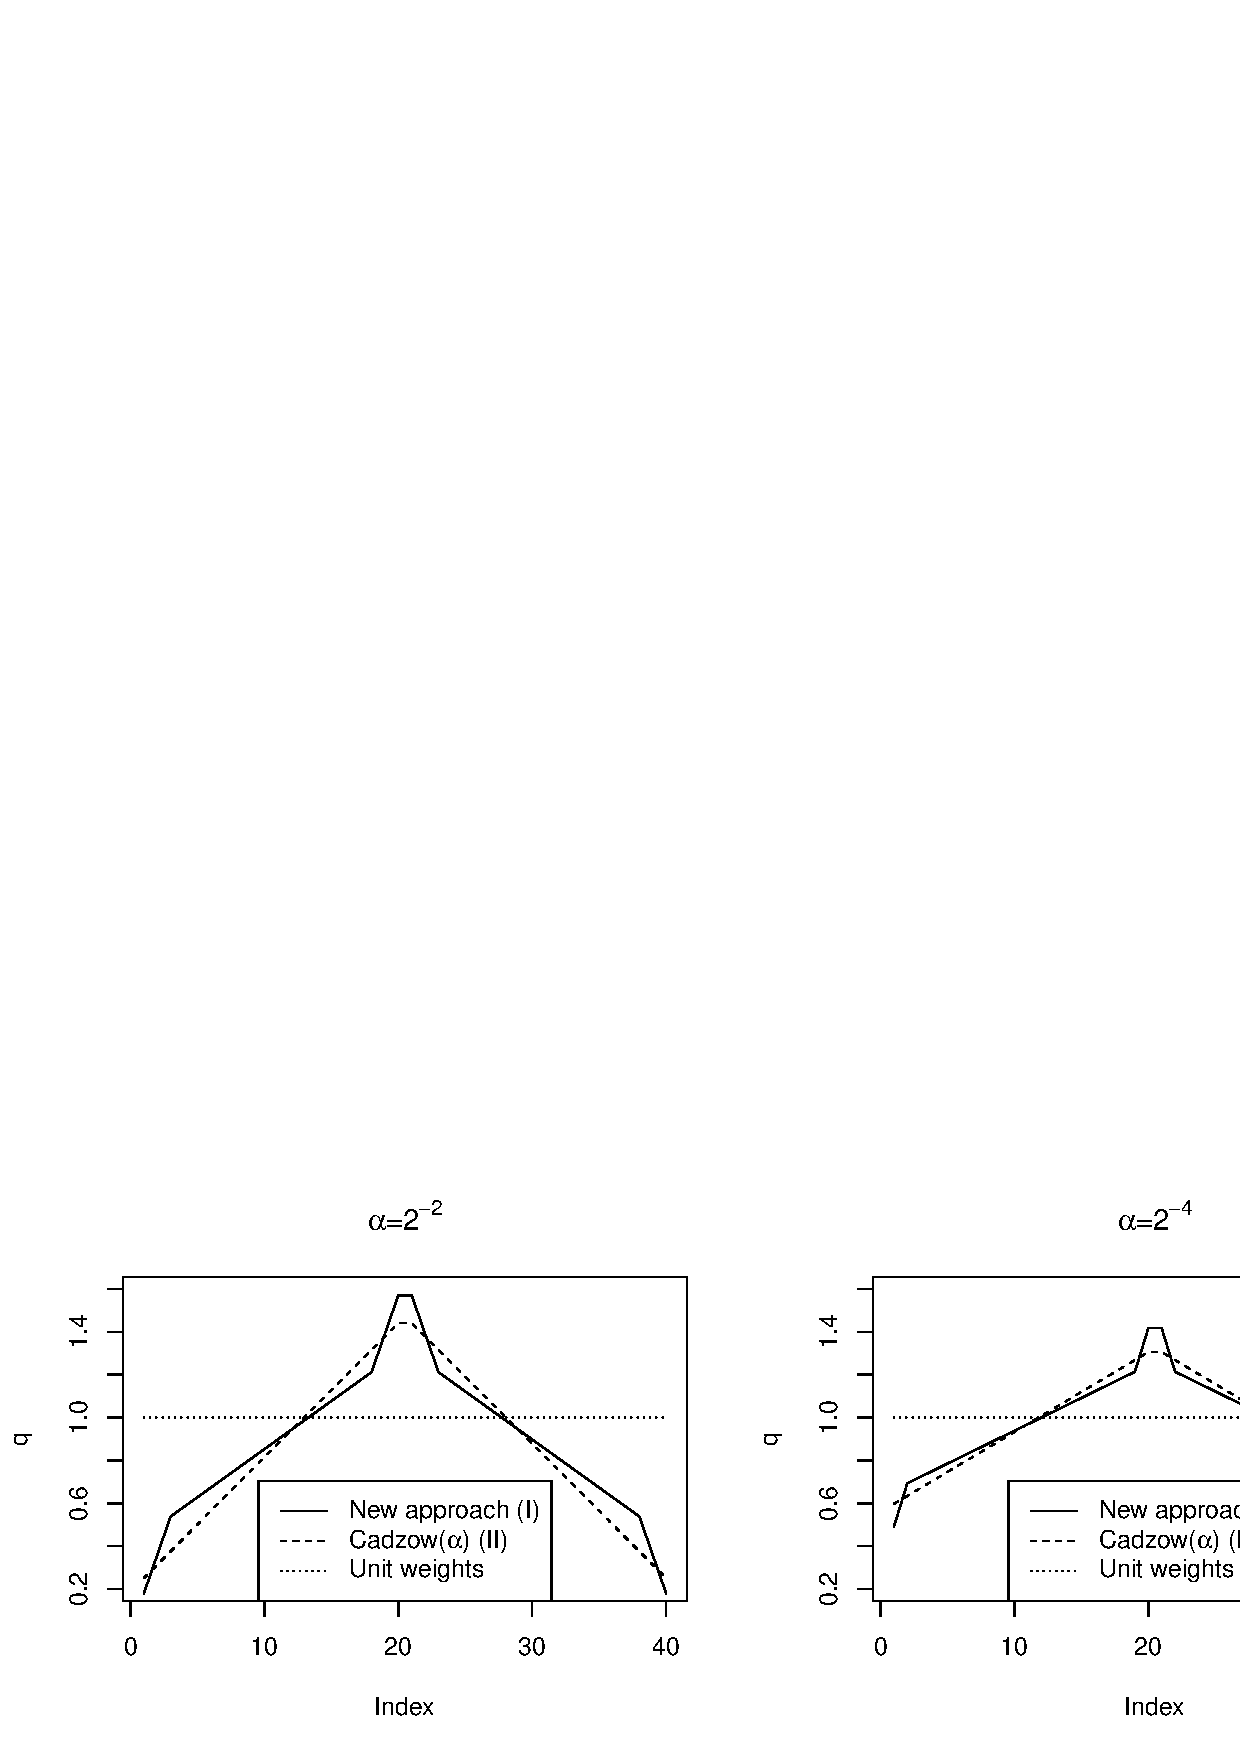
\includegraphics[width = 15cm]{weights.pdf}\caption{Веса ряда}\label{img_weights}
\end{center}\end{figure}
\subsection{Слабая разделимость}\label{weak_separ}
Введём еще одну характеристику алгоритмов, показывающую, насколько хорошо они раскладывают временной ряд на его аддитивные компоненты. Основным применением описанных алгоритмов является задача оценки сигнала, поэтому данное качество нам важно для получения как можно более точной оценки.

Пусть $\bfS \in \sfR^{K \times K}$ --- симметричная неотрицательно определённая матрица, $\tsX_1$ и $\tsX_2$ ---  два разных временных ряда длины $N$, $\bfX^1$, $\bfX^2$ --- их траекторные матрицы. Тогда \emph{коэффициентом корреляции $i$-го и $j$-го столбца} назовём следующую величину:
\begin{equation}\label{col_corr}
\rho^c_{i,j} = \frac{(X^1_i, X^2_j)}{||X^1_i|| ||X^2_j||},
\end{equation}
где $X^k_i$ --- $i$-й столбец матрицы $\bfX^k$, $k = 1, 2$, $(\cdot, \cdot)$ --- скалярное произведение, $||\cdot||$ --- евклидова норма. \emph{Коэффициентом корреляции $i$-й и $j$-й строки} назовём следующую величину:
\begin{equation}\label{row_corr}
\rho^r_{i,j} = \frac{(X^{1,i}, X^{2,j})_\bfS}{||X^{1,i}||_\bfS ||X^{2,j}||_\bfS},
\end{equation}
где $X^{k,i}$ --- $i$-я строчка матрицы $\bfX^k$, $k = 1, 2$, а $(\cdot, \cdot)_\bfS$ --- скалярное произведение с матрицей $\bfS$ в $\sfR^K$, определённая следующим образом: $(X, Y)_\bfS = ((X\bfS)^\sfT, Y^\sfT)$, так как $X$, $Y$ --- вектор-строчки, $|| \cdot ||_\bfS$ --- норма, порождённая этим скалярным произведением. Скажем, что ряды $\tsX_1$ и $\tsX_2$ \emph{слабо $\varepsilon$---разделимы}, если
\begin{equation}\label{weak_sep_eq}
\rho = \max(\max_{1 \le i,j \le K}|\rho^c_{i,j}|, \max_{1 \le i,j \le L}|\rho^r_{i,j}|) < \varepsilon.
\end{equation}
Нас будет интересовать порядок $\varepsilon$ при различных матрицах $\bfS$ и рядах $\tsX_1 = (c, c, \ldots)$ --- некоторая константа и $\tsX_2 = (\cos(2 \pi \omega k)), k = 1, 2, \ldots$, а так же при различных $L$ и $K$ при условии, что мы будем брать только $N = L + K - 1$ компонент ряда. Когда $\bfS$ --- единичная матрица, ответ известен: $\varepsilon$ имеет порядок $1/\min(L,K)$. Этот результат может быть найден в \cite{Golyandina.etal2001}.
\begin{lemma}
Пусть $\bfS$ определена аналогично Cледствию \ref{zhigconseq}:  Если $h = N/L$ --- целое, тогда  $\bfS$ --- диагональная матрица со следующими диагональными элементами:
\begin{equation*}
s_{k,k} = \begin{cases}
1, & \text{если} \quad k = jL+1 \quad \text{для некоторых} \quad j = 0, \ldots, h-1, \\
\alpha, & \text{в противном случае}
\end{cases},
\end{equation*}
где $0 \le \alpha \le 1$. Тогда $\rho$ имеет порядок $1/\min(L, N/L+\alpha(K - N/L))$ при $L, K \to \infty$.
\end{lemma}
\begin{proof}
Необходимо оценить порядки следующих величин:
\begin{gather*}
\rho^c_{i,j} = \frac{\sum_{k=j}^{j + L - 1} \cos(2 \pi \omega k)}{\sqrt{L (\sum_{k=j}^{j + L - 1} \cos^2(2 \pi \omega k))}},\\ \rho^r_{i,j} = \frac{\sum_{k=1}^K s_{k,k}\cos(2 \pi \omega (j + k - 1))}{\sqrt{(\sum_{k=1}^K s_{k,k}) (\sum_{k=1}^K s_{k,k}\cos^2(2 \pi \omega (j + k - 1)))}}.
\end{gather*}
Для доказательства используем следующие факты:
\begin{gather*}
\sum_{k=1}^n \cos(ak + b) = \csc(a/2) \sin(an / 2) \cos \left(\frac{an + a + 2b}{2} \right), \\
\sum_{k=1}^n \cos^2(ak + b) = \frac{1}{4}(\csc(a) \sin(2an + a + 2b) -\\ - \csc(a)\sin(a + 2b) + 2n),
\end{gather*}
для любых вещественных $a, b$ и положительного целого $n$.
Таким образом, когда ряд $\tsX_2$ не представляет из себя константу, числитель в $\rho^c_{i,j}$ имеет порядок $O(1)$, а знаменатель --- $O(L)$. Первая часть доказана, и её доказательство целиком аналогично случаю, когда $\bfS$ --- единичная матрица.

Для доказательства второй части необходимо разбить суммы и в числителе, и в знаменателе согласно соответствующим значениям $s_{k,k}$:
\begin{gather*}
\sum_{k=1}^K s_{k,k}\cos(2 \pi \omega (j + k - 1)) = \sum_{\substack{1 \le k \le K \\ s_{k,k} = 1}}\cos(2 \pi \omega (j + k - 1)) +\\ \sum_{\substack{1 \le k \le K \\ s_{k,k} = \alpha}}\alpha \cos(2 \pi \omega (j + k - 1)) = O(1) + \alpha O(1) = O(1),\\
\sum_{k=1}^K s_{k,k} = N/L + \alpha(K - N/L),\\
\sum_{k=1}^K s_{k,k}\cos^2(2 \pi \omega (j + k - 1)) = \sum_{\substack{1 \le k \le K \\ s_{k,k} = 1}}\cos^2(2 \pi \omega (j + k - 1)) +\\ \sum_{\substack{1 \le k \le K \\ s_{k,k} = \alpha}}\alpha \cos^2(2 \pi \omega (j + k - 1)) = O(N/L) + \alpha O(K - N/L).
\end{gather*}
\end{proof}
\emph{Замечание:} для выполнения леммы дополнительно требуется, чтобы ряды, составленные из элементов $(j, j + L, \ldots, (h-1)L + j)$, где $1 \le j \le L$, также не представляли из себя константу, что эквивалентно тому, что $\omega \ne k/L$ для любого целого $k$.

Таким образом, разделимость константы и синуса становится хуже, чем при обычном варианте: при $\alpha$, близких к нулю, оптимальным выбором $L$ будет $L \approx \sqrt{N}$, и, таким образом, получаем порядок разделимости $1/\sqrt{N}$.
\begin{lemma}
Пусть $\bfS$ определена аналогично Утверждению \ref{myweightstat}. Тогда $\rho$ имеет порядок $\max \left(1/L, \frac{H_L}{\sqrt{NK}} \right)$ при $L, K \to \infty$, где $H_L$ --- $L$-е гармоническое число.
\end{lemma}
\begin{proof}
Необходимо оценить порядки следующих величин:
\begin{gather*}
\rho^c_{i,j} = \frac{\sum_{k=j}^{j + L - 1} \cos(2 \pi \omega k)}{\sqrt{L (\sum_{k=j}^{j + L - 1} \cos^2(2 \pi \omega k))}}, \\ \rho^r_{i,j} = \frac{\sum_{k=1}^K \hat s_{k,k}\cos(2 \pi \omega (j + k - 1))}{\sqrt{(\sum_{k=1}^K \hat s_{k,k}) (\sum_{k=1}^K \hat s_{k,k}\cos^2(2 \pi \omega (j + k - 1)))}}.
\end{gather*}
Доказательство порядка для $\rho^c_{i,j}$ целиком аналогично предыдущему пункту, поэтому сразу перейдем ко второму. Докажем корреляцию только первых строчек --- для остальных доказательство будет целиком аналогичным. Рассмотрим числитель $\rho^r_{1,1}$:
\begin{gather*}
\sum_{k=1}^K \hat s_{k,k}\cos(2 \pi \omega k) = \sum_{k=1}^{L-1} \hat s_{k,k}\cos(2 \pi \omega k) + \sum_{k=L}^{K - L + 1} \frac{\cos(2 \pi \omega k)}{L} +\\ \sum_{k=K - L + 2}^{K} \hat s_{k,k}\cos(2 \pi \omega k) = I_1 + I_2 + I_3,
\end{gather*}
который разбился на три части. Для центральной справедлива оценка $O(1/L)$, а для левой части доказательство аналогично правой.
\begin{gather*}
\bigg|\sum_{k=1}^{L-1}\frac{1}{L}\left(\frac{k}{L} + \sum_{j=k}^{L-1} \frac{1}{j} \right) \cos(2 \pi \omega k)\bigg| = \bigg|\sum_{k=1}^{L-1} \frac{k \cos(2 \pi \omega k)}{L^2} + \\ + \frac{1}{L}\sum_{k = 1}^{L-1}\sum_{j = k}^{L-1}\frac{\cos(2 \pi \omega k)}{j}\bigg| \le 
\bigg|\sum_{k=1}^{L-1} \frac{k \cos(2 \pi \omega k)}{L^2}\bigg| + \bigg|\frac{1}{L}\sum_{k = 1}^{L-1}\sum_{j = k}^{L-1}\frac{\cos(2 \pi \omega k)}{j}\bigg|.
\end{gather*}
Используя тот факт, что
\begin{gather*}
\sum_{k=1}^n k \cos(ak + b) = -\frac{1}{4}\csc^2(a/2)(-(n+1)\cos(an+b) + \\ + n\cos(an + a + b) + \cos b),
\end{gather*}
получаем:
\begin{gather*}
\bigg|\sum_{k=1}^{L-1} \frac{k \cos(2 \pi \omega k)}{L^2}\bigg| = O(1/L), \quad
\bigg|\frac{1}{L}\sum_{k = 1}^{L-1}\sum_{j = k}^{L-1}\frac{\cos(2 \pi \omega k)}{j}\bigg| = \\ \bigg|\frac{1}{L}\sum_{j = 1}^{L-1}\sum_{k = 1}^{j}\frac{\cos(2 \pi \omega k)}{j}\bigg| \le \bigg|\frac{1}{L}\sum_{j = 1}^{L-1}\frac{\hat c}{j}\bigg| = O \left(\frac{H_L}{L} \right),
\end{gather*}
где $\hat c$ --- константа. Для знаменателя нужно рассмотреть следующие суммы:
\begin{equation*}
\sum_{k=1}^K \hat s_{k,k} = N / L
\end{equation*}
по определению, а следующую составляющую просто оценить снизу:
\begin{equation*}
\sum_{k=1}^K \hat s_{k,k}\cos^2(2 \pi \omega (j + k - 1)) \ge \sum_{k=1}^K \frac{1}{L}\cos^2(2 \pi \omega (j + k - 1)) = O \left(\frac{K}{L} \right).
\end{equation*}
\end{proof}
Для рядов $\tsX=(\sin(\frac{2 k \pi}{6}))$, $k = 1, \ldots 120$, и $\tsY = (1, 1, \ldots, 1)$ были посчитаны порядки слабой $\varepsilon$-разделимости при $L = 10, 20, 24, 30, 60$ и различных матрицах $\bfS$. Результат представлен на рисунке \ref{weakcorrimg}. Стоит заметить, что при небольших $L$ порядки слабой разделимости совпадают, потому что одинаковые для всех $\bfS$ корреляции столбцов по модулю больше, чем корреляции строк во всех случаях.
\begin{figure}[!h] \begin{center}
\includegraphics[width = 15cm]{weakcorr.pdf}\caption{Порядок слабой разделимости}\label{weakcorrimg}
\end{center}\end{figure}
\subsection{Небольшое исследование скорости алгоритма в применении к задаче очистки ряда от шума}
Для начала, следует ответить на некоторые оставшиеся вопросы. Первый из них --- в каком пространстве будет лежать результат работы алгоритма, если мы будем использовать $\bfS$ из леммы \ref{zhiglemma} при $\alpha = 0$.

Рассмотрим временной ряд $\tsX = (x_1, \ldots, x_N)$ длины $N \ge 3$. Зафиксируем длину окна $L$ $(1 < L < N)$ такую, что $N / L = h$ --- целое. Также рассмотрим последовательность векторов (непересекающиеся вектора вложения):
\begin{equation*}
\hat X_i = (x_{1 + (i-1)L}, \ldots, x_{iL})^\rmT, \qquad i = 1, \ldots, h.
\end{equation*}
\emph{Непересекающимся траекторным пространством} ряда $\tsX$ назовем $$\hat \spX^{(L)}(\tsX) = \hat \spX^{(L)} = \text{span}(\hat X_1, \ldots, \hat X_h).$$
\begin{definition}
%\begin{rank} \emph{
Пусть $0 \le r \le L$. Будем говорить, что ряд $\tsX$ \emph{имеет непересекающийся $L$-ранг $r$}, если $\dim \hat \spX^{(L)} = r$.
%}\end{rank}
\end{definition}

Заметим, что ряд $\tsX$ может иметь непересекающийся $L$-ранг $r$ только тогда, когда
\begin{equation}
r \le \min(L, h). \label{min_condition_nonint}
\end{equation}
Скажем, что при фиксированном $r$ длина окна $L$ является \emph{допустимой}, если для неё выполнено условие \eqref{min_condition_nonint}.

Тогда $\hat \sfX_N^r$ --- множество всех временных рядов длины $N$ непересекающегося $L$-ранга $r$ --- и есть множество, в котором будет лежать результат алгоритма. Важные замечания: во-первых, $\sfX_N^r \subset \hat \sfX_N^r$, так как соответствующие траекторные подпространства вкладываются друг в друга из-за того, что непересекающиеся вектора вложения являются подмножеством векторов вложения. Во-вторых, диагональное усреднение является биективным отображением --- усреднение происходит только по одной компоненте матрицы. Поэтому, алгоритм Cadzow при $\alpha = 0$ вырождается в одну операцию проектирования на матрицы меньшего ранга.

Следующий вопрос: достаточно хорошо ли устроено пространство $\hat \sfX_N^r$, чтобы проекцию на него использовать в качестве ответа на задачу об очистке зашумленного сигнала шума. Был взят следующий сигнал:
\begin{equation*}
\tsX = (x_{1}, \ldots, x_N), \qquad x_{i} = 5\sin{\frac{2 k \pi}{6}}, \quad k = 1, \ldots, N, \quad N = 40.
\end{equation*}
Алгоритмы запускались на следующем наборе рядов:
\begin{equation*}
\tsZ^j = \tsX + R_j^\rmT, \quad j = 1, \ldots, M, \quad M = 1000.
\end{equation*}
где каждый $R_j$ --- $N$ гауссовский белый шум с математическим ожиданием $0$ и дисперсией, равной $1$. Были взяты различные матрицы $\bfS$ и построена оценка отклонения от $\tsX$ при различном числе итераций. Параметры: $L = 8$ (соответственно, $h = 5$), $r = 2$. Результаты представлены на рисунке \ref{img_cadzowspeed}.
\begin{figure}[!h] \begin{center}
\includegraphics[width = 15cm]{cadzowspeed.pdf}\caption{Оценка отклонения от $\tsX$ при различном числе итераций}\label{img_cadzowspeed}
\end{center}\end{figure}

Видно, что при $\alpha = 0$ оценка, построенная проекцией на $\hat \sfX_N^r$, является достаточно плохой. При $\alpha$, близких к нулю, алгоритм на первой итерации дает ряд, достаточно близкий к $\hat \sfX_N^r$, но в дальнейшем алгоритм сходится к хорошей оценке, но с низкой скоростью: чем ближе $\alpha$ к нулю, тем медленнее сходимость. Дополнительно, был проведён эксперимент с $L_1 = 8$ и $L_2 = 20$, где результаты размещены на одном рисунке \ref{img_cadzowspeed2}. Видно, что чем меньше $L$, тем ближе веса к единичным, но, с другой стороны, падает скорость сходимости.

\begin{figure}[!h] \begin{center}
\includegraphics[width = 15cm]{cadzowspeed_2.pdf}\caption{Оценка отклонения от $\tsX$ при различном числе итераций и различных $L$}\label{img_cadzowspeed2}
\end{center}\end{figure}

\section{Сходимость алгоритмов}
Для новых введенных алгоритмов еще не показаны свойства, касающиеся их сходимости. Известный результат для базового алгоритма может быть найден в \cite{Cadzow1988}. Рассмотрим общий случай. Для этого нам понадобятся следующие утверждения:
\begin{proposition} \label{pythaprop}
Пусть $X$ --- гильбертово пространство, $\calM$ --- замкнутое относительно умножения на скалярную величину подмножество ($x \in \calM \Rightarrow \alpha x \in \calM \, \forall \alpha \in \sfR$), $\Pi_\calM$ --- оператор проектирования на $\calM$ \footnote{На самом деле, проекция может быть определена неоднозначно, но дальше будем предполагать, что оператор однозначен. В данном случае, можно выбирать любой вариант для проекции, это никак не влияет на истинность утверждений.}. Тогда для любого $x \in X$ выполняется теорема Пифагора: $||x||^2 = ||x - \Pi_\calM x||^2 + ||\Pi_\calM x||^2$.
\end{proposition}
\begin{proof}
Представим множество $\calM$ в виде $\calM = \bigcup\limits_{l \in L}l$, где $L$ --- множество всех прямых, лежащих в $\calM$ и проходящих через $0$, и $l \cap m = 0$ для любых $l, m \in L$, $l \neq m$. Тогда операция проектирована может быть записана так: вначале мы выбираем прямую $l$ такую, что $\text{dist}(x, l) \rightarrow \min\limits_{l \in L}$, после чего $y = \Pi_\calM x$ --- это проекция $x$ на $l$. Получаем нужное свойство.
\end{proof}

Теперь рассмотрим $\sfR^{L \times K}$, множество матриц ранга, не превосходящего ранга $r$ $\calM_r$, множество ганкелевых матриц $\calH$, при этом нас устроит любая порожденная скалярным произведением метрика, $\Pi_{\calM_r}$ и $\Pi_\calH$ --- проекторы на соответствующее пространства в зафиксированной метрике. Более того, все утверждения справедливы и для траекторных псевдоматриц в алгоритме Extended Cadzow. Пусть $\bfX_0 \in \calH$, $\bfX_k = \Pi_\calH \Pi_{\calM_r} \bfX_{k - 1}$, $k = 1, 2, \ldots$
\begin{proposition}\label{chuprop}
\cite{Chu2003} Справедливы следующие неравенства:
\begin{equation*}
||\bfX_k - \Pi_{\calM_r} \bfX_k|| \ge ||\Pi_{\calM_r} \bfX_k - \bfX_{k + 1}|| \ge ||\bfX_{k+1} - \Pi_{\calM_r} \bfX_{k + 1}||.
\end{equation*}
\end{proposition}
\begin{proof}
Для проектора $\Pi_\calH$ справедливо:
\begin{equation*}
||\Pi_{\calM_r} \bfX_k - \bfX_{k + 1}|| = ||\Pi_{\calM_r} \bfX_k - \Pi_\calH \Pi_{\calM_r} \bfX_k|| \le ||\Pi_{\calM_r} \bfX_k - \bfY||
\end{equation*}
для любого $\bfY \in \calH$, в частности, и для $\bfY = \bfX_k$. Оставшееся неравенство доказывается аналогично.
\end{proof}

\begin{proposition}
В топологии, порожденной фиксированной метрикой (эквивалентной порожденной фробениусовской нормой) множество матриц $\calM_r$ ранга, не превосходяего $r$, является замкнутым. \footnote{Для алгоритма Extended Cadzow $\calM_r$, вообще говоря, не является даже множеством матриц, но оно является непрерывной проекцией замкнутого множества матриц ранга, не превосходящего $r$, порядка $L \times N + L - 1$.}
\end{proposition}
\begin{proof}
Опустим случай, когда $r = \min(L, K)$ --- тогда $\calM_r = \sfR^{L \times K}$, и оно очевидно замкнуто.

Возьмем матрицу $\bfX \in \sfR^{L \times K}$. Если её ранг больше $r$, тогда существует квадратная подматрица порядка $r+1$, определитель которой не равен нулю. Если же ранг меньше, либо равен $r$, то определители всех таких подматриц равны нулю.

Построим следующее отображение: 
\begin{equation*}
f(\bfX) = \sum \limits_{\bfY in \sfY} |\det \bfY|,
\end{equation*}
где $\sfY$ --- множество всех подматриц матрицы $\bfX$ порядка $r + 1$. Заметим, что по построению $f$ --- непрерывное отображение.

Теперь рассмотрим любую сходящуюся последовательность из $\calM_r$: $\bfX_1$, $\bfX_2$, $\ldots$, $\bfX^*$ --- предельная точка. Знаем, что для любого $k = 1, 2, \ldots$: $f(\bfX_k) = 0$. Пользуясь непрерывностью отображения $f$ получаем, что $f(\bfX^*) = 0$. А это означает то, что $\bfX^* \in \calM_r$.
\end{proof}
\begin{theorem}
\begin{enumerate}
\item $||\bfX_k - \Pi_{\calM_r}\bfX_k|| \to 0$ при $k \to +\infty$, $||\Pi_{\calM_r}\bfX_k - \bfX_{k+1}|| \to 0$ при $k \to +\infty$.
\item Существует сходящаяся подпоследовательность $\bfX_{i_1}, \bfX_{i_2}, \ldots$ такая, что ее предел $\bfX^*$ лежит в $\calM_r \cap \calH$.
\end{enumerate}
\begin{proof}
\begin{enumerate}
\item Согласно утверждению \ref{chuprop}, последовательности $(||\bfX_k - \Pi_{\calM_r} \bfX_k||)$ и $(||\Pi_{\calM_r} \bfX_k - \bfX_{k + 1}||)$, $k = 1, 2, \ldots$ являются невозрастающими. Очевидно, они ограничены снизу нулём. Поэтому они имеют одинаковый предел $c$, опять же согласно \ref{chuprop}.

Докажем, что $c = 0$. Предположим противное: существует $d > 0$ такое, что для любого $k = 1, 2, \ldots$: $||\bfX_k - \Pi_{\calM_r} \bfX_k|| > d$, $||\Pi_{\calM_r} \bfX_k - \bfX_{k + 1}|| > d$. Согласно утверждению \ref{pythaprop}, справедливо следующее:
\begin{gather*}
||\bfX_k||^2 = ||\Pi_{\calM_r} \bfX_k||^2 + ||\bfX_k - \Pi_{\calM_r} \bfX_k||^2 =\\ ||\bfX_k - \Pi_{\calM_r} \bfX_k||^2 + ||\Pi_{\calM_r} \bfX_k - \bfX_{k + 1}||^2 + ||\bfX_{k + 1}||^2.
\end{gather*}
Таким образом, $||\bfX_{k+1}||^2 < ||\bfX_k||^2 - 2d^2$. Расписывая неравенство аналогично дальше, получим, что для любого $j = 1, 2, \ldots$: $||\bfX_{k+j}||^2 < ||\bfX_k||^2 - 2 j d^2$. Возьмём любое $k$, например $k = 1$, и $j = \lceil ||\bfX_k||^2 / (2d^2) \rceil + 1$. Тогда $||\bfX_{k+j}||^2 < 0$, чего не может быть.
\item Рассмотрим последовательность $(\Pi_{\calM_r} \bfX_k)$, $k = 1, 2, \ldots$. Она ограничена, так как $||\Pi_{\calM_r} \bfY|| \le ||\bfY||$ и $||\Pi_{\calH} \bfY|| \le ||\bfY||$ для любого $\bfY \in \sfR^{L \times K}$ (это справедливо, например, и по утверждению \ref{pythaprop}). Тогда мы можем выбрать из неё сходящуюся подпоследовательность $(\Pi_{\calM_r} \bfX_{i_k})$, $\bfX^*$ --- её предел, при этом $||\Pi_{\calM_r} \bfX_{i_k} - \bfX_{i_k + 1}|| = ||\Pi_{\calM_r} \bfX_{i_k} - \Pi_\calH \Pi_{\calM_r} \bfX_{i_k}|| \to 0$ при $k \to + \infty$. Учитывая, что $||\bfY - \Pi_\calH \bfY||$ --- композиция непрерывных отображений, получаем, что $||\bfX^* - \Pi_\calH \bfX^*|| = 0$ и зная, что $\calM_r$ --- замкнутое множество, получаем, что $\bfX^* \in \calM_r \cap \calH$. Осталось увидеть, что последовательность $(\Pi_\calH \Pi_{\calM_r} \bfX_{i_k})$ --- сходящаяся, так как $\Pi_\calH$ --- непрерывное отображение, и ее предел равен $\bfX^*$. Получаем, что $\bfX_{i_k + 1}$ --- требуемая подпоследовательность.
\end{enumerate}
\end{proof}
\end{theorem}
\section{Исследование алгоритмов в задаче восстановления рядов и подведение итогов}
Была произведена проверка набора известных алгоритмов для приближения временных рядов в задаче восстановлении рядов. Важно понимать, мы наблюдаем зашумленные ряды, и к зашумлённым рядам применяем алгоритмы, пытаясь оценить именно исходный ряд.
Исследуемые ряды имеет вид:
\begin{equation*}
\tsX = (x_1, \ldots, x_N), \qquad x_k = 5\sin{\frac{2 k \pi}{6}}, \quad k = 1, \ldots, N, \quad N = 40.
\end{equation*}
\begin{gather*}
\tsY = (y_1, \ldots, y_N), \qquad y_k = 5\sin{\frac{2 (k + 2/3) \pi}{6}} e^{k / 20}, \\ k = 1, \ldots, N, \quad N = 40.
\end{gather*}
Алгоритмы запускались на следующем наборе рядов:
\begin{gather*}
\tsZ^1_j = \tsX + R_j^\rmT, \quad j = 1, \ldots, M, \quad M = 1000, \\
\tsZ^2_j = \tsY + R_j^\rmT, \quad j = 1, \ldots, M, \quad M = 1000.
\end{gather*}
где каждый $R_j$ --- гауссовский белый шум длины $N$ с математическим ожиданием $0$ и дисперсией, равной $1$. При этом везде выбрано $r=2$, а оптимальной шириной окна во всех случаях оказалось $L = 20$.

Для каждого алгоритма было рассмотрено:
\begin{itemize}
\item Используемые веса ряда $q_i$
\item $P$ --- оценка среднеквадратического отклонения до $\tsX$ или $\tsY$ (оценивание сигнала) на одной итерации алгоритма
\item $P$ --- оценка среднеквадратического отклонения до $\tsX$ или $\tsY$ (оценивание сигнала) на  большом ($T = 100$) числе итераций.
\item Трудоёмкость
\end{itemize}

\subsubsection{Алгоритм Cadzow при $\alpha$ = 1}
\begin{itemize}
\item Имеет веса $q_i = w_i$, описанные в \eqref{hankel_weight}.
\item $P = 0.3749$ для ряда $\tsX$ и $P = 0.3762$ для ряда $\tsY$ на одной итерации алгоритма. Алгоритм хорошо работает на одной итерации благодаря хорошим свойствам слабой разделимости рядов.
\item $P = 0.3714$ для ряда $\tsX$ и P = $0.3661$ для $\tsY$ на ста итерациях.
\item Алгоритм быстро сходится и не требует дополнительных итераций для проектирования на множество матриц неполного ранга.
\end{itemize}

\subsubsection{Алгоритм Cadzow при $\alpha$ = 0.1}
\begin{itemize}
\item Имеет веса $q_i$, описанные в Следствии \ref{zhigconseq}.
\item $P = 0.4312$ для ряда $\tsX$ и $P = 0.4434$ для ряда $\tsY$ на одной итерации алгоритма. Не самые лучшие результаты объясняются плохой слабой разделимостью рядов.
\item $P = 0.3254$ для ряда $\tsX$ и P = $0.3220$ для $\tsY$ на ста итерациях. Хорошие результаты объясняются близкими к единичным весами.
\item Алгоритм не требует дополнительных итераций для проектирования на множество матриц неполного ранга, однако чем меньше $\alpha$, тем медленнее он сходится.
\end{itemize}

\subsubsection{Алгоритм Cadzow с матрицей $\hat{\bfS}$}
\begin{itemize}
\item Имеет веса $\hat q_i$, описанные в Утверждении \ref{myserweightstat}.
\item $P = 0.3643$ для ряда $\tsX$ и $P = 0.3718$ для ряда $\tsY$ на одной итерации алгоритма.
\item $P = 0.3494$ для ряда $\tsX$ и P = $0.3439$ для $\tsY$ на ста итерациях.
\item Алгоритм быстрый и не требует дополнительных итераций для проектирования на множество матриц неполного ранга. Практически не уступает основному алгоритму Cadzow.
\end{itemize}

\subsubsection{Алгоритм Weighted Cadzow}
\begin{itemize}
\item Имеет веса $q_i = 1$ для любого $i = 1, \ldots, N$.
\item $P = 0.3640$ для ряда $\tsX$ и $P = 0.3734$ для ряда $\tsY$ на одной итерации алгоритма, но серьёзно ``притягивается'' на краях шумом.
\item $P = 0.3393$ для ряда $\tsX$ и P = $0.3343$ для $\tsY$ на ста итерациях.
\item Алгоритм требует дополнительные итерации для проектирования на множество матриц неполного ранга, поэтому достаточно медленный.
\end{itemize}

\subsubsection{Алгоритм Extended Cadzow}
\begin{itemize}
\item Имеет веса $q_i = 1$ для любого $i = 1, \ldots, N$ (но целевая функция не в точности соответствует исходной, так как рассматривается расширенный ряд).
\item $P = 0.3330$ для ряда $\tsX$ и $P = 0.3474$ для ряда $\tsY$ на одной итерации алгоритма. Может ``притягиваться'' на краях шумом.
\item $P = 0.3171$ для ряда $\tsX$ и P = $0.3191$ для $\tsY$ на ста итерациях. Алгоритм очень нестабилен для нестационарных рядов, если в качестве оценки скрытых переменных брать среднее по исходному ряду, а не использовать векторное прогнозирования.
\item Алгоритм требует дополнительные итерации для проектирования на множество матриц неполного ранга, и вследствие своей специфики, очень медленный.
\end{itemize}
Изображения, на которых показана ошибка восстановления в точке для различных рядов и методов, представлены ниже. Оценки среднеквадратичного отклонения собраны в таблицу \ref{fintable}.

\begin{table}[!h]
\begin{center}
\caption{Сравнение алгоритмов}\label{fintable}
\begin{tabular}{|c|c|c|c|c|}
\hline
$P$: & $\tsX$, $T = 1$ & $\tsY$, $T = 1$ & $\tsX$, $T = 100$ & $\tsY$, $T = 100$  \\
\hline
Cadzow, $\alpha = 1$ & 0.3749 & 0.3762 & 0.3714 & 0.3661 \\
\hline
Cadzow, $\alpha = 0.1$ & 0.4312 & 0.4434 & 0.3254 & 0.3220 \\
\hline
Cadzow $\hat{\bfS}$ & 0.3643 & 0.3718 & 0.3494 & 0.3439 \\
\hline
Weighted Cadzow & 0.3640 & 0.3734 & 0.3393 & 0.3343 \\
\hline
Extended Cadzow & 0.3330 & 0.3474 & 0.3171 & 0.3191 \\
\hline
\end{tabular}
\end{center}
\end{table}

\begin{figure}[!h] \begin{center}
\includegraphics[width = 15cm]{s1_it1.pdf}\caption{Ошибка восстановления в точке на одной итерации для ряда $\tsX$}
\end{center}\end{figure}
\begin{figure}[!h] \begin{center}
\includegraphics[width = 15cm]{s2_it1.pdf}\caption{Нормированная ошибка восстановления в точке на одной итерации для ряда $\tsY$}
\end{center}\end{figure}
\begin{figure}[!h] \begin{center}
\includegraphics[width = 15cm]{s1_it100.pdf}\caption{Ошибка восстановления в точке на ста итерациях для ряда $\tsX$}
\end{center}\end{figure}
\begin{figure}[!h] \begin{center}
\includegraphics[width = 15cm]{s2_it100.pdf}\caption{Нормированная ошибка восстановления в точке на ста итерациях для ряда $\tsY$}
\end{center}\end{figure}

\clearpage
\section*{Заключение}
\addcontentsline{toc}{section}{Заключение}
Таким образом, в работе были рассмотрены и исследованы разные методы решения задачи выделения сигнала, управляемого ЛРФ. Также, было проведено численное сравнение методов.

Перечислим вкратце полученные в результате исследований итоги:
\begin{itemize}
\item Weghted Cadzow и Extended Cadzow --- очень трудоёмкие алгоритмы, в то время как основной алгоритм и его модификации, использующие косоугольное SVD-разложение, примерно одинаково быстры.
\item Чем меньше $L$, тем веса $q_i$ ближе к единичным, и алгоритмы сходятся к лучшему ответу.
\item Чем меньше $L$, тем скорость сходимости меньше; чем больше $L$, тем скорость сходимости выше.
\item Для алгоритма Cadzow при различных $\alpha$: при $\alpha = 0$ имеем сходимость не к тому множеству рядов, при $\alpha > 0$ --- сходимость к рядам конечного $L$-ранга есть, но чем меньше $\alpha$, тем она медленнее.
\item
В рассмотренных примерах, на одной итерации лучшим оказался трудоёмкий благодаря внутренним итерациям метод Extended Cadzow для длины окна порядка половины длины ряда.
В пределе лучшим оказался самые медленно-сходящиеся методы Cadzow($\alpha$) при маленьком $\alpha$ и маленькой длине окна.
\end{itemize}

\bibliographystyle{plain}

\bibliography{ssa2012}
\end{document}